% -*- TeX:UTF-8 -*-
%%
%% KAIST 학위논문양식 LaTeX용 (ver 0.4) 예시
%%
%% @version 0.4.1
%% @author  채승병 Chae,Seungbyung (mailto:chess@kaist.ac.kr)
%% @date    2004. 11. 12.
%% @modifier 신호철 (mailto:h.c.shin@kaist.ac.kr)
%% @moddate 2018. 11. 29
%%
%% @requirement
%% teTeX, fpTeX, teTeX 등의 LaTeX2e 배포판
%% + 은광희 님의 HLaTeX 0.991 이상 버젼 또는 홍석호 님의 HPACK 1.0
%% : 설치에 대한 자세한 정보는 http://www.ktug.or.kr을 참조바랍니다.
%%
%% @note
%% 기존에 널리 쓰여오던 차재춘 님의 학위논문양식 클래스 파일의 형식을
%% 따르지 않고 전면적으로 다시 작성하였습니다. 논문 정보 입력부분에서
%% 과거 양식과 다른 부분이 많으니 아래 예시에 맞춰 바꿔주십시오.
%%
%%
%% @acknowledgement
%% 본 예시 논문은 물리학과 박사과정 김용현 님의 호의로 제공되었습니다.
%%
%% -------------------------------------------------------------------
%% @information
%% 이 예제 파일은 hangul-ucs를 사용합니다. UTF-8 입력 인코딩으로
%% 작성되었습니다. hlatex의 hfont는 이용하지 않습니다. --2006/02/11
%% 본 템플릿은 전산학부 김민혁 교수에의해서 버그 수정되었습니다. -- 2016/11/25
%% 전자과 신호철에 의해서 포맷 수정됨 (주로 draft 버전에서의 논문 표시양식)

% @class kaist.cls
% @options [default: doctor, korean, final]
% - doctor: 박사과정 | master : 석사과정
% - korean: 한글논문 | english: 영문논문
% - final : 최종판   | draft  : 시험판
% - pdfdoc : 선택하지 않으면 북마크와 colorlink를 만들지 않습니다.

%indicator for the final version
%N.B. Use \finaltrue for dissertation publication, and use \finalfalse for the proposal and defense
\newif\iffinal
\finaltrue %to set final marker as true -> final
%\finalfalse %set final marker as false -> draft

\iffinal
	\documentclass[master,english,final,pdfdoc]{kaist-ucs-improved}
	\usepackage{lmodern} %This suppresses font size warnings in final version
\else
	\documentclass[master,english,draft,pdfdoc]{kaist-ucs-improved}

\fi


\usepackage{array}
\usepackage{numprint}
\usepackage{multirow}
\usepackage{booktabs}
\usepackage{threeparttable}
\usepackage{amsmath}
\usepackage{listings}
\usepackage{shortcuts}
%% \usepackage{listing}
%% \usepackage{equation*}

%\setcounter{secnumdepth}{1}

%Enable numbering upto subsubsection
%Increase the number to enable numbering for lower levels: e.g. \paragraph and \subparagraph
\setcounter{secnumdepth}{3}

%Line breaking for long URL's (line is broken also by '-')


\def\UrlBreaks{\do\/\do-\do\_}

% If you want make pdf document (include bookmark, colorlink)
%\documentclass[doctor,english,final,pdfdoc]{kaist-ucs}

% kaist.cls 에서는 기본으로 dhucs, ifpdf, graphicx 패키지가 로드됩니다.
% 추가로 필요한 패키지가 있다면 주석을 풀고 적어넣으십시오,
%\usepackage{...}

% @command title 논문 제목(title of thesis)
% @options [default: (none)]
% - korean: 한글제목(korean title) | english: 영문제목(english title)
\title[korean] {위임 지분 증명 방식 가상화폐의 리소스 관리 위협 분석(이오스 자원관리 시스템 취약점 분석)}
\title[english]{Why Decentralized resource management is difficult: vulnerability analysis of resource utilization of EOS.IO}

% @note 표지에 출력되는 제목을 강제로 줄바꿈하려면 \linebreak 을 삽입.
%       \\ 나 \newline 등을 사용하면 안됩니다. (아래는 예시)
%
%\title[korean]{탄소 나노튜브의 물리적 특성에 대한\linebreak 이론 연구}
%\title[english]{Theoretical study on physical properties of\linebreak
%                carbon nanotubes}
%
% If you want to begin a new line in cover, use \linebreak .
% See examples above.
%


% @command author 저자 이름
% @param   family_name, given_name 성, 이름을 구분해서 입력
% @options [default: (none)]
% - korean: 한글이름 | chinese: 한문이름 | english: 영문이름
% 한문 이름이 없다면 빈 칸으로 두셔도 됩니다.
%
%
% If you are a foreigner , write your name in korean or your korean name.
% If you can't write native character, you can make the chinese blank empty 
% Write as follow
% \author[korean]{family name in korean}{given name in korean}
% \author[chinese]{family name in your native language}{given name in your native language}
% \author[english]{family name in english}{given name in english}
%
\author[korean]{이}{상 섭}
\author[korean2]{이}{상섭}    %이름을 붙여 써 주시기 바랍니다.
\author[chinese]{}{} %Don't want hanja
\author[english]{Lee}{Sangsup}

% @command advisor 지도교수 이름 (복수가능)
% @usage   \advisor[options]{...한글이름...}{...영문이름...}{signed|nosign}
% @options [default: major]
% - major: 주 지도교수  | coopr: 공동 지도교수
\advisor[major]{김용대}{Yongdae Kim}{signed}
\advisor[major2]{김용대}{Yongdae Kim}{signed} %한글 성과 한글 이름을 모두 붙여 써 주시기 바랍니다.
%\advisor[coopr]{손수엘}{Sooel Son}{}
%\advisor[coopr2]{손수엘}{Soo-el Son}{} 
\advisorinfo{Professor of Electrical Engineering} %제출승인서에 들어가는 교수님 정보, advisor's information  
%Yongdae
%For final draft
%\advisor[coopr]{홍 길 동}{Gil-Dong Hong}{nosign}
%\advisor[coopr2]{홍길동}{Gil-Dong Hong}{nosign}    %한글 성과 한글 이름을 모두 붙여 써 주시기 바랍니다.
%
% 지도교수 한글이름은 입력하지 않아도 됩니다.
% You may not input advisor's korean name
% like this \advisor[major]{}{Chang, Kee Joo}{signed}


% @command department {학과이름}{학위종류} - 아래 규칙에 따라 코드를 입력
% @command department {department code}{degree field}
%
% department code
% 2. 석박사학위논문 작성 및 제출요령 4쪽 ~ 5쪽 참고
% 또는 kaist-ucs.cls 의 % @command department 참고

% science: 이학 | engineering: 공학 | business : 경영학
% 박사논문의 경우는 학위종류를 입력하지 않아도 됩니다.
% If you write Ph.D. dissertation, you cannot input degree field.
% The third parameter : a | b | c
% a: 소속된 학과만 쓰는 옵션 (학과에만 소속되어 있는 경우에는 무조건 a를 선택해야 함)
% b: 학과 아래의, 프로그램이나 학제전공에 소속되어 있을 경우에 학과와 프로그램을 함께 쓰는 옵션
% c: 학과 아래의, 프로그램이나 학제전공에 소속되어 있을 경우에 학과를 쓰지 않고 프로그램이나 학제전공의 이름만 쓰는 옵션 
% 
% a: it represents only the name of department. (if you aren't in the program under the department, must choose a)
% b: it represents the names of department and the program that is under the department (consider this when you are in the program not only department)
% c: it represents only the name of program that is under the department (consider this when you are in the program not only department)

\department{AA}{engineering}{Information Security}

% @command studentid 학번(ID)
\studentid{20183410}

% @command referee 심사위원 (석사과정 3인, 박사과정 5인)
\referee[1]{김 용대}
\referee[2]{류 석영}
\referee[3]{손 수엘}
%\referee[4]{정}
%\referee[5]{무}
% \referee[5] {Barack Obama}
% Of course english name is available

% @command approvaldate 지도교수논문승인일
% @param   year,month,day 연,월,일 순으로 입력
\approvaldate{2019}{12}{17} %SHOULD BE MODIFIED 
%\fontsize{17.28pt}{17.28pt}\selectfont %Font size changed from 18pt to 17.28pt to remove warnings

% @command refereedate 심사위원논문심사일
% @param   year,month,day 연,월,일 순으로 입력
\refereedate{2019}{12}{17} %SHOULD BE MODIFIED

% @command gradyear 졸업년도
\gradyear{2020} %SHOULD BE MODIFIED



% 본문 시작
\begin{document} 

    % 앞표지, 속표지, 학위논문 제출승인서, 학위논문 심사완료 검인서는
    % 클래스 옵션을 final로 지정해주면 자동으로 생성되며,
    % 반대로 옵션을 draft로 지정해주면 생성되지 않습니다.
    % 학위논문 제출 승인서에서 자신의 전공과 교수님의 정보를 바꾸기 위해서는 첨부되어있는 제목이 kaist-ucs인 class 문서에 들어가서 ####################로 표시  
    % 한 부분을 바꾸시길 바랍니다.

    % 논문 서지, 초록, 핵심 낱말, 영문 초록, 영어 핵심 낱말 (Information of thesis, abstract in korean, keywords in korean, abstract in english, keywords in english)
    %% 한글 초록은 500자를, 영문 초록은 300 낱말을 넘지 않아야 함
    %% 핵심 낱말은 5 개 이내로 넣음
    %% 한글 초록에 영문 글자를 쓰지 않도록 한다.
		\thesisinfo
   
    %\begin{summary}      
    %지난 10여 년간 탄소 나노튜브는 자체의 독특한 전기적, 기계적 성질로
    %인하여 다가오는 나노기술 분야의 이상적인 기초물질중의 하나로 떠오르고
    %있다. 흑연을 감는 세세한 방법에 따라 전기적 특성이 금속성에서 1eV의
    %띠간격을 가지는 반도체 특성까지 다양한 분포로 존재한다.
    %본 학위논문에서는 탄소 나노튜브의 여러 물리적 성질에 대해 고찰하는데,
    %기본적으로 제일원리 밀도함수 이론과 밀접결합근사 모형을 사용하여 전기적
    %특성과 그 제어 방법, 자기적 특성, 그리고 수송특성 등을 다루고자 한다.
    %\end{summary}
   
    %\begin{Korkeyword}
    % 가, 나, 다
    %\end{Korkeyword}

		%Locate abstract in a separate file
		% ABSTRACT
\begin{abstract}
\EOS is a popular cryptocurrency, whose market cap is over seven billion USD.
Its ecosystem operates in the \PLATFORM system, which is devised to speed up the
slow transaction rate of previous blockchain technologies.
%
Whereas many previous studies have investigated the security issues of \btc and
\eth, the security of \PLATFORM has thus far drawn little attention despite
its popularity.
%
Even the studies that have addressed the security of EOS and its underlying
blockchain system mostly focused on implementational bugs in the core of
the \PLATFORM system or in smart contracts, rather than addressing the
fundamental problems stemming from the \eos design.

To address this void in the previous literature, we investigate the design
architecture of \eos. Based on this investigation, we introduce four attacks
whose root causes stem from the unique characteristics of \eos, including
intentionally slowing down the block creation time---which can disrupt the
essential functions of its blockchain and incapacitate the entire \eos system.
%
In addition, we find that an adversary can partially freeze the execution of
a target smart contract or maliciously consume all the resources of a target
user with crafted requests.
%
We report all the identified threats to the \eos foundation, one of which
is confirmed to be fatal.
%
Finally, we discuss possible mitigations against the proposed attacks.

\end{abstract} 

% KEYWORD
\begin{Engkeyword}
	EOS, EOS.IO, Resource, Security, Vulnerabilities
\end{Engkeyword}
\newpage




		
\begin{abstract2}

이오스는 시가총액이 70억 달러가 넘는 인기있는 암호 화폐이다. 이오스는 이전 다른 블럭체인의 느린 거래속도를 보완하고자 고안 되었으며 이오스 생태계는 이오스.아이오 시스템에서 작동한다. 하지만 이오스의 많은 인기에도 불과하고 이전의 연구들은 비트코인 및 이더리움의 보안 연구에 촛점이 맞추어져 있으며, 현업에서의 이오스 보안의 경우에도 스마트컨트랙트의 구현상의 오류에만 주로 촛점이 맞추어져 있다. 이 논문에서는 이전의 이러한 연구의 공백을 해결하기 위해 이오스닷.아이오의 설계적 취약점을 조사하고, 이 조사를 바탕으로 이오스닷 아이오의 고유한 특성을 이용한 4가지 공격을 소개한다. 본 논문에서 소개할 공격은 블럭체인의 필수 기능을 못 사용 하게끔 만들 뿐만 아니라 블럭 생성시간을 의도적으로 느리게 하여 전체 이오스닷아이오 시스템이 작동하지 않을 수 있다. 또한 공격자는 대상 스마트 컨트랙으의 실행을 부분적으로 중지 시키거나 대상 사용자의 모든 리소스를 악의적인 요청으로 모두 소모 시킬수 있다. 확인된 모든 위협은 이오스닷 아이오의 설립자에게 보고되었으며 그중 하나는 치명적인 버그로 명명되어 즉각 패치 되었다. 이 논문에서는 위 4가지 공격을 소개하고 공격에 대한 완화 방법에 대해 논의한다.

\end{abstract2}

\begin{Engkeyword2}
	이오스, 이오스닷아이오, 리소스, 보안, 취약점
\end{Engkeyword2}

    \addtocounter{pagemarker}{1}                 % 백색별지분을 고려
    \newpage  
  
		\iffinal
			% 목차 (Table of Contents) 생성
			\tableofcontents

			% 표목차 (List of Tables) 생성
			\listoftables

			% 그림목차 (List of Figures) 생성
			\listoffigures
		\else
			\label{paperlastromanpagelabel} %For removing warning in draft mode
			\pagenumbering{arabic} % Draft mode has no pagenumbering so add it.
		\fi

    % 위의 세 종류의 목차는 한꺼번에 다음 명령으로 생성할 수도 있습니다.
    %\makecontents
%% 한글로 쓴 논문에는 본문에 영문 글자를 쓰지 않는다. 다만, 꼭 필요할 때에는 ‘한글 낱말 (영문 낱말)’ 꼴로 적는다.
%% 이하의 본문은 LaTeX 표준 클래스 report 양식에 준하여 작성하시면 됩니다.
%% 하지만 part는 사용하지 못하도록 제거하였으므로, chapter가 문서 내의
%% 최상위 분류 단위가 됩니다.
%% You cannot use 'part'

		%Chapters in separate files
		\chapter{Introduction} %Don't want chapter number for intro

Recently, \textit{cryptocurrency} has attracted a great deal of attention due
to its rapidly growing market cap. Bitcoin, often called the first
cryptocurrency, reached a market cap of over 100 billion USD in 2019, and more
than 2K cryptocurrencies have emerged worldwide, thus representing a combined
value of over 200 billion USD~\cite{coincap}. This surging interest in the
cryptocurrency has also attracted the attention of both industry and
academia for its underlying \textit{blockchain} system. Consequently, many
studies have been conducted to analyze and improve the core technology of each
blockchain system~\cite{\bcPapers}.

The security of the blockchain is another important issue for which vast
research has been conducted. These studies focused on analyzing double
spending~\cite{karame2012double}, network-related
attacks~\cite{heilman2015eclipse, apostolaki2017hijacking},
illicit transactions~\cite{son2019ndss}, transaction
malleability~\cite{decker2014bitcoin, andrychowicz2015malleability}, selfish
mining~\cite{\miningpoolPapers}, or smart contracts~\cite{\smartcontractAll}.
However, most of these studies have only focused on the two major
cryptocurrencies; \btc and \eth.

\eos is an emerging blockchain system, whose cryptocurrency, \EOS, possesses a
market cap of over seven billion USD~\cite{coincap}, making it one of the top
five cryptocurrencies worldwide.~\footnote{
We checked this at the time of the submission.}
%
There have been only a few studies on its security~\cite{\eosBugs}.
%
The \eos foundation has been incentivizing researchers through a bug bounty
program, but most of the bugs found so far are related to implementation, such
as software vulnerabilities that an adversary can exploit to perform
arbitrary code execution~\cite{\eosSoftwareBugs}, or logical bugs that cause a
smart contract to deviate from the objectives of its developers
~\cite{\eosSCBugs}. However, as the design of \eos is markedly different from
that of \btc or \eth in managing system resources, there may exist distinctive
and unexplored threats that stem from the resource management policies of the \eos
system.

To address the lack of research in this area, we chose \eos as the objective of
this study and analyzed its security.
%
We first studied the characteristics of the \eos system. Note that some parts
of the \eos whitepaper~\cite{EOSWHITEPAPER} are outdated or ambiguous; hence,
we had to manually analyze the source code to figure out its actual implemented
semantics.

To speed up the slow transaction rate of previous blockchain systems, \eos
adopted a \textit{Delegated Proof of Stake (DPoS)} algorithm~\cite{
larimer2014delegated}, which delegates the consensus on blocks and execution of
the smart contracts to the representative nodes, called Block Producers (\BPs).
%\kirhanote{EOS가 DPoS를 대표하는 코인이라는 말을 추가하면 어떨까요?}
This design decision of using DPoS entails problems of sharing computational
resources among a small number of \BPs. To effectively manage resources and
prevent resource abuse, \eos asks a participant to obtain a resource capacity,
such as computational power, network bandwidth, and storage~\cite{
EOSWHITEPAPER}.
%
Even though this new means of resource management can effectively support the
representative nodes in executing smart contracts, it raises new concerns about
added assets that can negatively impact the security of the
system~\cite{howard2006security}.


% Important of resource managements.
Any attack on resource managements that leads to a denial of service (DoS) is a
critical security threat. Many emerging blockchain systems strive to achieve 
high Transactions-Per-Second (TPS) rate, which enables the provision of a
short-latency service for their users and service providers. Incessant attacks
that successfully undermine the availability or TPS of blockchain services break
fundamental requirements that blockchain service users expect. For instance,
stock transaction services or payment services at retail stores demand a short
latency to process financial transactions. Exacerbating transaction time
directly affects the quality of these services, thus contributing to users
choosing other blockchain services.


Therefore, we investigated resource-related threats that exploit the design
architecture unique to \eos. We manifested the capabilities of smart contract
providers (SCPs) as well as their service users and defined an \eos adversary
who is able to conduct the same level of privileged operations as these
participants do. Under this adversary model, we identified four possible attack
scenarios: \NODEDOS, \TESER, \SCPDOS, and \TOCTOU attacks.
%
In these attacks, an adversary intentionally incapacitates the entire \eos system
with a crafted smart contract, an adversary depletes or drains the resources of
a smart contract provider so that this victim no longer provides the service,
and a malicious smart contract provider surreptitiously replaces the original smart
contract with another one to steal user assets.

In order to address these attacks, we analyze their causes and propose several
mitigations. These mitigations include simple preventative measures along with
suggestions for systematic changes of \eos. We believe that the proposed
mitigations can prevent the attacks described in this paper as well as potential
future threats.

In summary, our contributions are as follows:
\begin{itemize}
\item We present the \emph{block delay} attack, a novel attack that exploits
    a transaction scheduling policy of the \eos system. This attack is able
    to delay all transactions in the system, thus resulting in the DoS.
\item We introduce two new attack methods: \emph{\TESER and \SCPDOS} attacks.
    These attacks exploit resource management policies unique to the system,
    thus disrupting services from a target smart contract provider.
\item We present the \emph{\TOCTOU} attack scenario that abuses controversial
    design decisions of the system. The attack allows locking \ram resources
    of a target user, which enables an attacker to ask a ransom in exchange for
    releasing the locked \ram resources.
\item We demonstrate the feasibility of each attack and estimate the impact of
    each proposed attack scenario based on experiments conducted in a local \eos
    system.
\item We propose preventative measures as well as a redesign of the \eos system
    to mitigate the proposed and potential threats.
\end{itemize}


		\chapter{Background}
\label{s:back}

\section{\eos overview}
\label{ss:overview}

\begin{figure}[!t]
  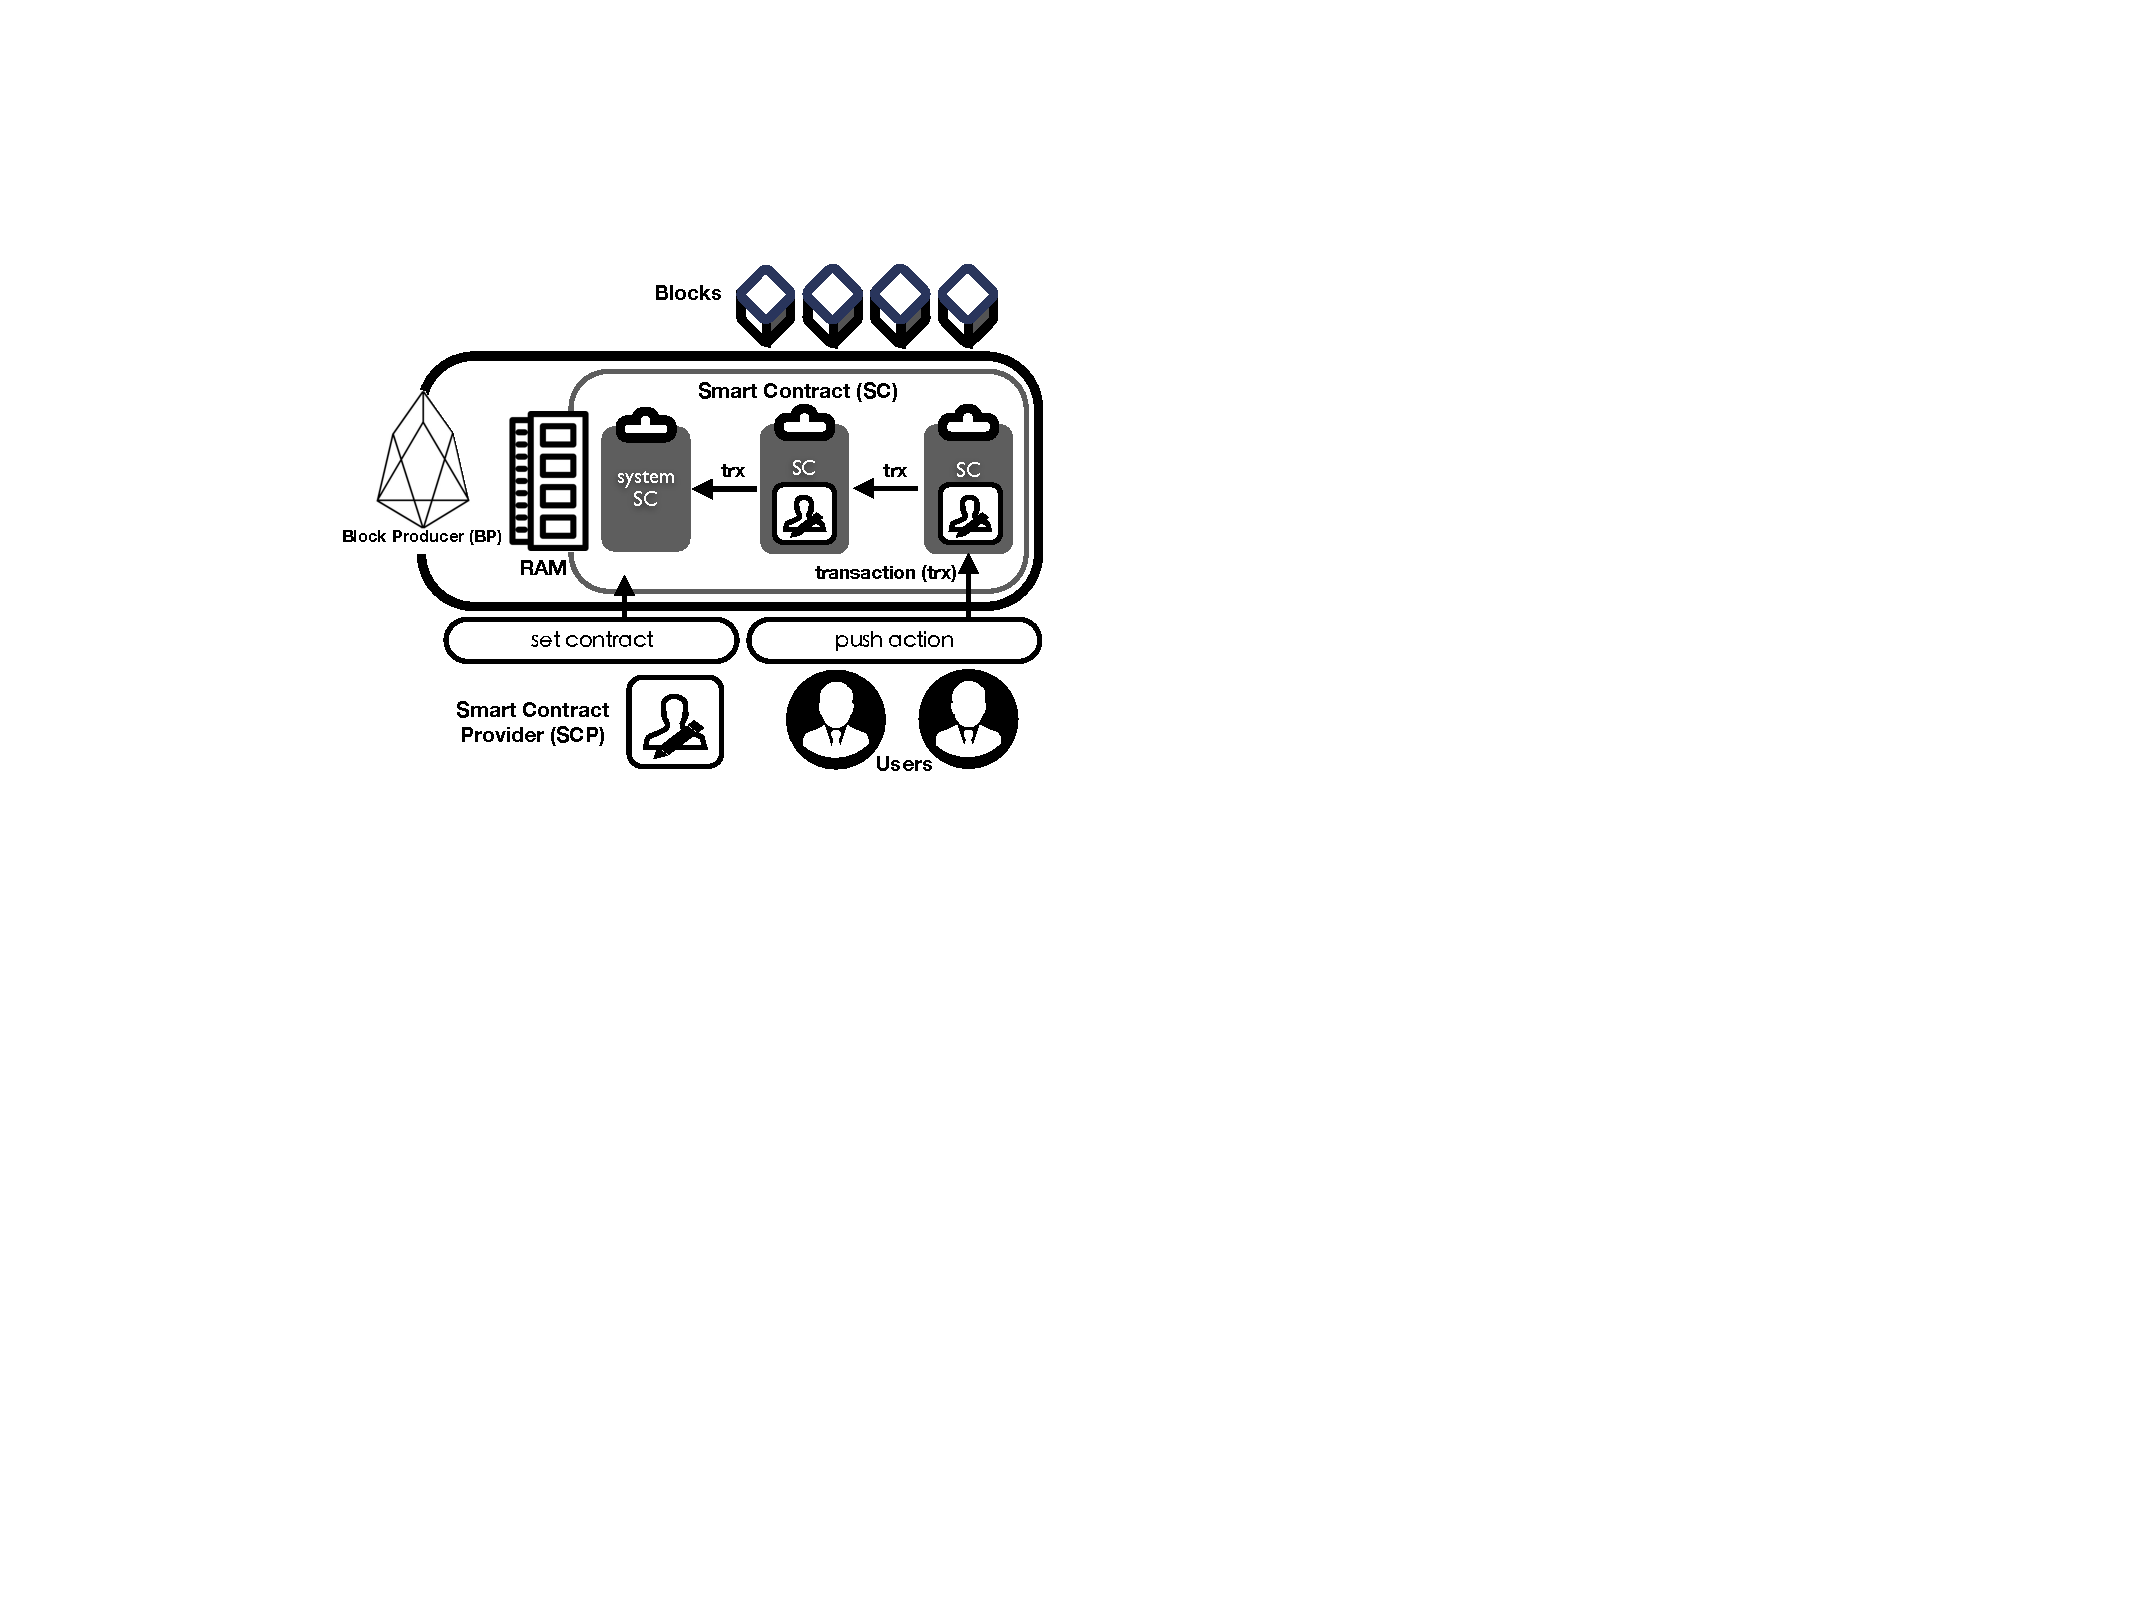
\includegraphics[width=\linewidth]{figures/philosophy.pdf}
  \caption{Architecture of \PLATFORM}
  \label{fig:overview}
\end{figure}

% What is EOS.
\eos is a blockchain system for a cryptocurrency called EOS. In this section, we
describe the main characteristics of \eos. As some parts of its
whitepaper~\cite{EOSWHITEPAPER} are outdated and ambiguous, we interpret them
based on our judgment by carefully analyzing the \eos source code.
%and referring this article~\cite{xueos}.
%
~\autoref{fig:overview} illustrates a simplified overview of the \eos ecosystem.
%
The main difference between \eos and the other blockchain systems lies in its
consensus algorithm, which is the core of the blockchain system.
%
Unlike the other blockchain systems of the top cryptocurrencies in the
market~\cite{coincap}, \eos adopted \textit{Delegated Proof of Stake
(DPoS)}~\cite{larimer2014delegated} as its consensus algorithm. DPoS delegates
the role of a node in a blockchain system to a small number of representative
nodes, known as \textit{Block Producers (\BPs)}.
%
Among the nodes in the \eos network, 21 BPs are selected through a voting
procedure; these BPs are responsible for deciding whether newly created blocks
can be attached to the current chain.
%
With DPoS, \eos is able to significantly speed up its transaction rate.

Another feature of \eos is its ability to execute a \textit{smart contract
(\SC)}, which is essentially a program developed by a user. It is similar to
those supported by the \eth platform~\cite{wood2014ethereum}. In this paper,
we call the developers of \SCs as \textit{Smart Contract Providers (\SCPs)}.
%
In the \eos system, if a user wants to execute an SC, s/he can send a
\textit{transaction} to one of the BPs in the \eos network.
%
This transaction consists of several \textit{actions} that specify a target
\SC and the parameters for the execution of the \SC.
%
%If the recipient node is not a BP, the transaction is finally transferred to
%one of the BPs.
When the \BP receives the transaction, it executes the requested \SC after
fetching the SC from the \eos chain and creates a new \eos block that stores
the execution results. Then, the new block is propagated to the other BPs
through a broadcasting procedure.



\section{\eos smart contract}
\label{ss:contract}
% 컨트랙트가 수정 가능한 배경 제시
An \SC often refers to a computer program that executes on a blockchain system
or a distributed ledger. Many blockchain ecosystems, including \eth and \eos,
support the execution of a given SC for various purposes, including banking,
gambling, initial coin offerings (ICOs), and trading in the marketplace~\cite{
dappradar}.

The design of \eth, the most popular blockchain system that supports \SCs,
demands that every \SC in their system should be unchangeable; thus, it allows
no revision not even for updating the source code or fixing vulnerabilities in
the \SCs. Therefore, \SCPs, in practice, dispose of their \SCs and create new
ones in order to patch inherent bugs.

On the other hand, \eos allows \SCPs to modify their \SCs. However, this design
decision entails another problem that \SCPs are able to change the semantics of
their \SCs, which are then executed by users without any active notification of
the change.
%
Therefore, users have few options but to completely trust \SCPs to execute their
\SCs while understanding that these \SCs may be changed at any time.

The option still remains for users to analyze an \SC to understand its semantics
before executing the \SC; however, \SCs in the \eos system are binary programs
compiled in the form of \textit{Web Assembly}~\cite{bastien2015webassembly},
which makes the understanding of their semantics difficult.
%
Furthermore, \SCPs are under no responsibility to open the source code of
their \SCs. According to one of the \eos explorers called EOS Park, only
10\% of \SCPs release their source code publicly~\cite{eospark}.
%
These characteristics of \eos make it difficult for users to analyze each \SC,
further contributing to users having no choice, but to trust the goodwill of \SCPs.



\section{Resources of \eos}
\label{ss:stake}

Every transaction and execution involving SCs in the \eos system consumes
resources.
%
By design, the system abstracts its resources into three items: computational
power, network bandwidth, and storage. For convenience, in this paper, we call
these as \cpu, \net, and \ram, respectively.
%
When a user directs a transaction to run an SC, the user should already have
enough resources for the consumption by the SC, called \textit{transaction costs}.
%
Therefore, the platform asks participating SCPs and users to purchase \ram or
to stake \cpu and \net.
%
Here, \emph{staking} refers to an action of allocating a certain number of EOS
tokens (i.e., EOS cryptocurrency) to reserve BP resources.

\eos adopted this mechanism to effectively manage the constrained resources of
the BPs and prevent resource abuse.
%
More specifically, when a user stakes EOS tokens, \eos distributes the capacity
of the resources to a user proportional to the tokens staked by this user.
%
For example, if a user staked 1\% of the total staked EOS tokens, then the user
is allowed to use 1\% of the total resource capacity as well.
%
Staked tokens do not disappear but are marked as staked in the system. That is,
a user can unstake his/her tokens anytime, and the tokens become available after
three days. At the time of unstaking, the staked \cpu and \net are also
released.
%
On the other hand, the tokens of the purchased \ram are not returned. \ram is 
storage for the data used within an SC, and the user can refund \ram only if the
data used in the target SC is removed.
%
Therefore, a user should consider using his/her resources wisely.





\section{\EOS resource payment}
\label{ss:receiver}

The underlying design philosophy for \eos is \emph{Receiver Pays}, denoting that
SCPs should pay for the usage of their SCs by users.
%
More specifically, a user only pays for the initial transaction cost, while the
SCP pays for the other costs of the subordinate transactions which come within
the first SC.
%
Consequently, the costs of running SCs become the business costs for which 
SCPs should be responsible. SCPs stake their \cpu and \net for the users who 
execute their SCs, and the amount of staked resources strongly affects the 
number of processed transactions from users.

However, it is burdensome for those SCPs who require a large amount of \cpu and
\net to execute their SCs. In such cases, SCPs can delegate the resource usage to
users.
%
Even though \eos enables the SCPs to delegate the transaction costs to the
users, it requires an additional permission, called the \code, from the users. If
this permission is given, an SCP can control all the resources of a user,
including EOS tokens.
%`
As a result, since most users would not want to give their permission to an
SCP, many SCPs follow the Receiver Pays model by paying for the business costs
during the execution of their SCs.

		\chapter{Attack Model}

We assume an \eos adversary who utilizes the same functionalities of the \eos
system as \SCPs and their service users do.
%
That is, the adversary is able to implement and manage her own SCs, or to
execute other SCs.
%
The adversary can also entice victims to send a transaction that triggers the
execution of a crafted SC.
%
Furthermore, the adversary is capable of updating the crafted \SC anytime to
leverage the misplaced trust of the victims who only examined the previous SC
before the update.
One goal of the adversary is to deplete available resources of \SCPs, such as
\cpu, \net, or \ram, thus causing the denial of service (DoS) for these \SCPs.
The adversary also aims to cause delays in block generation in BPs,
because such delays significantly undermine the service availability of the \eos
system.
%
Consider SCs for stock trading or banking services, which demand a short latency
for task completion. In such services, any system delay can potentially
lead to a significant financial loss as transactions that should be
processed within a short time cannot be processed.
%
Furthermore, the adversary could also plunder the resources of the victims and
demands a ransom.

Note that our adversary model is similar to those used in the previous studies
that exploit \SC bugs~\cite{\smartcontractPapers} in \eth or cause double 
spending in \btc with spam transactions~\cite{blockproblem}, except that the 
adversary is able to update the crafted \eos \SC.


		\chapter{Attacks}

We present four novel attacks against the \eos system. The \NODEDOS
(\S\ref{label_reentrancy-attack}) attack undermines service availability of \BPs,
thus contributing to block generation delays in the \eos system.
%
The \TESER (\S\ref{label_teser}) and \SCPDOS (\S\ref{SCPDOS}) attacks deplete the
resources staked for the execution of \SCs, including \cpu and \ram, thus
resulting in the denial of \SC services.
%
The \TOCTOU (\S\ref{label_toctou}) attack exploits the controversial \EOS design
decision that allows \SC updates. The adversary starts by obtaining the
sensitive permission with her benign \SC code and then changes it later to
deplete the \ram of the victims. The adversary may then ask a ransom for
releasing victims' \ram.
%
We emphasize that all the presented attacks harness attack vectors unique to
\eos.

In this section, we describe each attack and demonstrate its feasibility with an
attack experiment that measures its potential impact on \PLATFORM.
%

\PP{Experimental setup.}
We conducted experiments to measure how much loss each attack can cause in
\PLATFORM. We used a machine running 64-bit Ubuntu 16.04.3 LTS with Intel Core
i7-8700 CPU at 3.20 GHz (12 cores), 32 GB of RAM, and 200 GB SSD.
%
For the testing environment, we prepared two different versions of \eos on the
machine: version 1.1.1, where we discovered the \NODEDOS attack, and version
1.7.3, which is the latest stable version to confirm the patch for the \NODEDOS
attack and to test the feasibility of other attacks.
%
Each version of \eos is initialized with default system SCs that manage the
resources of \eos and the execution of other SCP-provided SCs.
%
Note that we have never conducted the presented attacks against the actual \eos
system in production for ethical and respectable research.

\PP{Collected SCs.}
We collected 3,212 \SCs from 3,600 accounts in the \eos main network
and installed them in our testing environment.





\section{Block delay attack}
\label{label_reentrancy-attack}
The \NODEDOS attack causes a delay in the production of blocks in a \BP by
generating an unacceptable number of spurious transactions. These spurious
transactions elicit misbehaviors in the \BP when scheduling them, thus usurping
opportunities that should have been used for processing valid transactions.
This entails huge financial losses for participants in \PLATFORM by delaying
the transactions that require immediate completion.
%
We note that this attack targets all \SCs running in \BPs, not a
particular \SC, which makes the attack even more critical.

A DoS on any blockchain system is indeed a critical security threat, as many
emerging blockchain systems strive to provide a high-availability service with
a high TPS.
%
Because the \eos system only depends 21 representative \BPs to process worldwide transactions, the DoS on a single \BP may cause a significant TPS degradation.
%
We first describe the \eos block generation procedures and then explain how
the \NODEDOS attack exploits the procedures.



\begin{figure}[!t] %%%% t->h or ht
\centering
  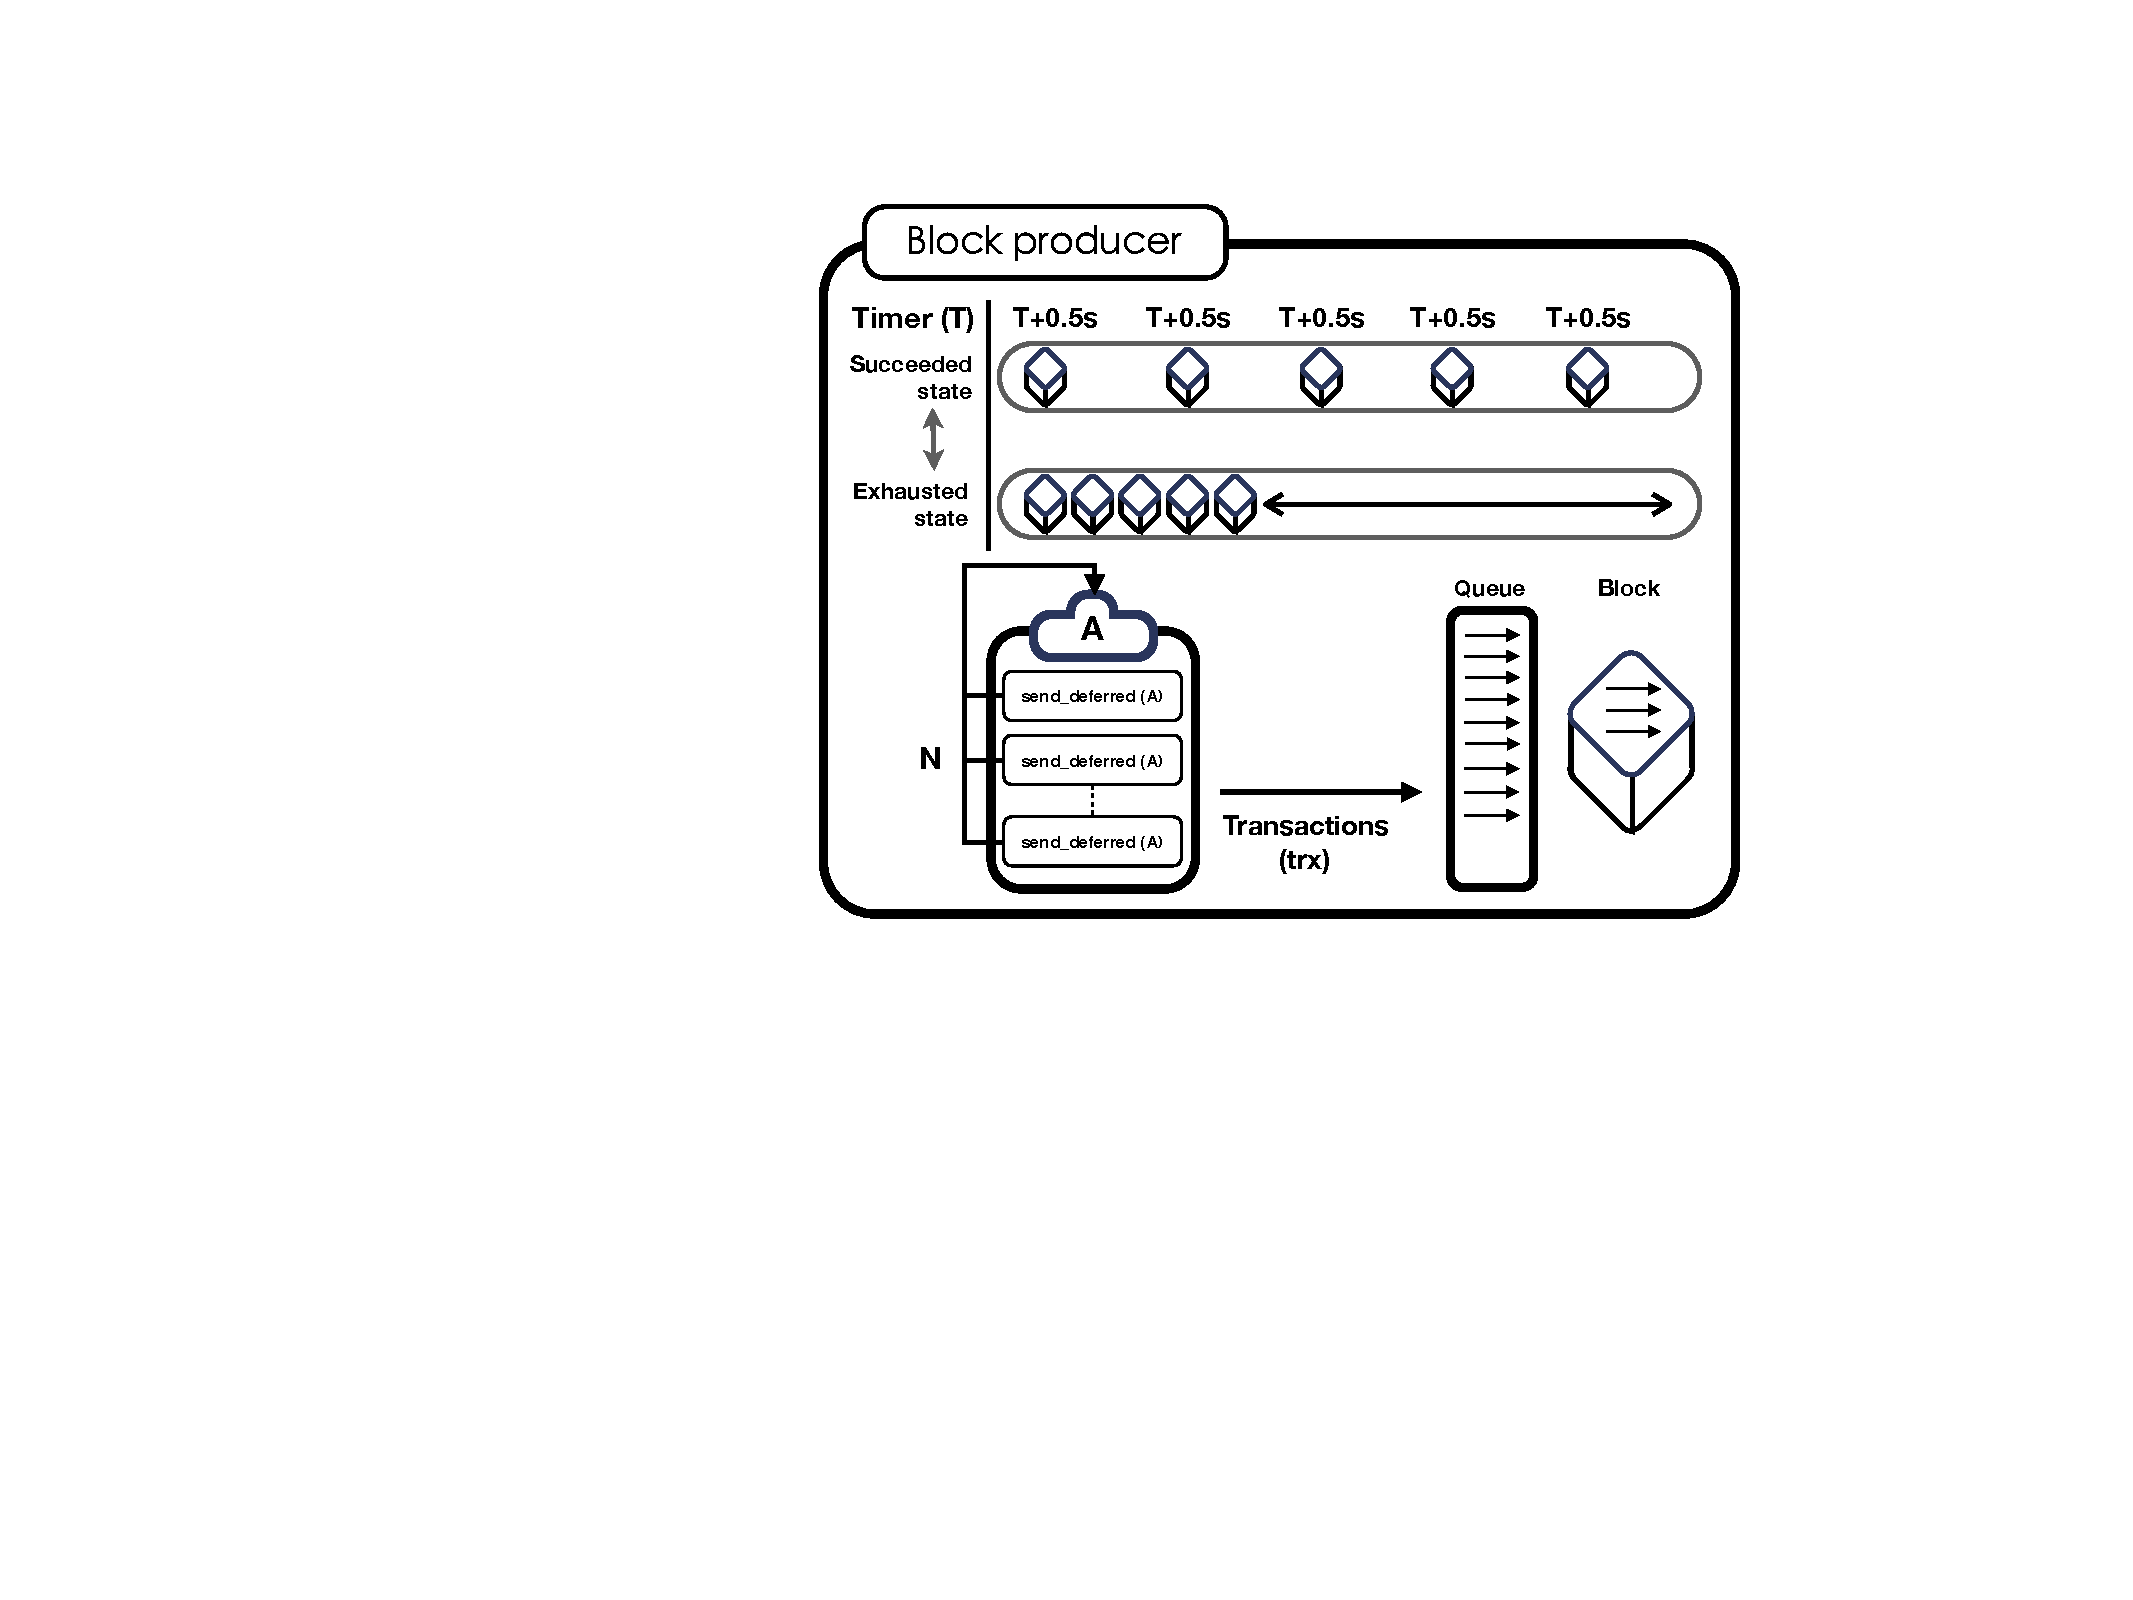
\includegraphics[width=0.9\linewidth]{figures/BlockDOS.pdf}
  \caption{Overview of the \NODEDOS attack.}
  \label{fig:pow}
\end{figure}

\PP{Block generation procedures.}
The \eos system has two internal policies; 1) a \BP should generate a block
within every 0.5 seconds; 2) a \BP limits its resource usage for processing
transactions within a block. Specifically, \eos limits the execution time as
well as the amount of \cpu and \net for processing transactions within a single
block.

To enforce these block generation policies, \eos has four internal states,
including \textit{succeeded} and \textit{exhausted} states. We only explain
these two states relevant to initiate the \NODEDOS attack.
%
In the succeeded state, a \BP generates a block for every 0.5 seconds. When a
\BP completes given transactions earlier than 0.5 seconds, it waits further and
then propagates the resulting block to other \BPs.
%
If the resource usage for processing transactions within a block is over a
specified threshold, it switches its state to the exhausted state and generates
as many blocks as possible without any waiting time to maximize its computation
resources.

A block generation delay arises when the exhausted state is changed back to the
succeeded state after a large number of blocks are generated in the exhausted
state. This delay stems from the time gap between the timestamp specified in a
block and the actual time when the block is generated. For each block, \eos
specifies a timestamp with the multiplication of the fixed time interval (0.5
seconds) with the number of all generated blocks in the entire \eos system that
precede the current block. That is, a \BP in the exhausted state could create a
block of which timestamp indicates a future time, when the \BP creates more than
one block within 0.5 seconds.
%
When the state is changed back to the succeeded state, the \BP attempts to
generate a new block with a future timestamp. It then pauses its block
generation until the real time matches the timestamp of this new block.


\PP{Attack conditions.}
In order to intentionally invoke such a block generation delay, the attack
should 1) change the succeeded state to the exhausted state, 2) make the \BP to
generate a large amount of blocks in the exhausted state, and then 3) change the
\BP back to the succeeded state.

By carefully analyzing the \eos system, we found that an adversary could easily
conduct the \NODEDOS attack by abusing two \eos features:
deferred transactions, and smart contract updates.

In general, a \BP executes a requested transaction right away, however, a
deferred transaction is scheduled later for its execution~\cite{EOSWHITEPAPER}.
The original purpose is to move computations into different shards or to create
a long-running process for continuance transactions.
%
To initiate a deferred transaction, an \SC invokes \texttt{send\_deferred()},
which makes a new asynchronous transaction on a \BP. Suppose an adversary
implements a malicious \SC that recursively invokes multiple deferred
transactions of itself. The execution of this \SC causes an exponentially
increasing number of crafted transactions, as~\autoref{fig:pow} illustrates.

When a \BP receives such a large number of transactions, its resources
eventually runs out and the \BP changes its state to the exhausted state.

After producing numerous transactions, an adversary changes the crafted \SC to a
totally different one. This change renders all the queued transactions from the
original \SC invalid because those transactions still attempt to call methods in
the original \SC which no longer exists.
%
Therefore, the \BP in the exhausted state marks the spurious transactions as
invalid and immediately process them, thereby generating a large amount of
blocks.
%
Consequently, these spurious blocks generates a huge gap between the timestamp
of the last block and the real time. When the \BP comes back to the succeeded
state, the \BP pauses its further block generation.
%
Consider that a \BP generates each one of 100 blocks for 0.2 seconds in the
exhausted state, thus taking 20 seconds ($0.2 * 100$). The timestamp of the last
block must be set to 50 seconds ($0.5 * 100$), thereby producing the time gap of
30 seconds. As a result, the \BP should delay its next block generation for 30
seconds when the state changes back to the succeeded one.
%
As the adversary is able to manage the number of blocks with the deferred
transaction, she can impose an arbitrary delay time, resulting in the DoS of
the \BP under the attack.



\begin{table}[!t]
\centering
\setlength\tabcolsep{0.07cm}
\caption{Estimated financial loss by the \NODEDOS attack}
\label{tab:nodedos_eval}

\begin{threeparttable}
\begin{tabular}{@{}rrcccrccr@{}}
\toprule

\multirow{2}[6]{*}{\textbf{\begin{tabular}[c]{@{}c@{}} Block \\ Count \end{tabular}}} &
&
\multicolumn{4}{c}{\textbf{Attacker}} &
&
\multicolumn{2}{c}{\textbf{Victim}}
\\
\cmidrule{3-6}
\cmidrule{8-9}
&
&
\multicolumn{1}{c}{\begin{tabular}[c]{@{}c@{}} Time\tnote{$\dagger$} \\ (min)\end{tabular}} &
\multicolumn{1}{c}{\begin{tabular}[c]{@{}c@{}} \cpu \\ (min)\end{tabular}} &
\multicolumn{1}{c}{\begin{tabular}[c]{@{}c@{}} \net \\ (MiB)\end{tabular}} &
\multicolumn{1}{c}{\begin{tabular}[c]{@{}c@{}} Cost\tnote{$\ddagger$} \\ (EOS)\end{tabular}} &
&
\multicolumn{1}{c}{\begin{tabular}[c]{@{}c@{}} Delay \\ (min)\end{tabular}} &
\multicolumn{1}{c}{\begin{tabular}[c]{@{}c@{}} Loss\tnote{$\ast$} \\ (EOS)\end{tabular}}
\\
\midrule
376   &  & 0.92    & 1.23  & 16.13   & 480   &  & 2.05 & 40,802  \\
704   &  & 2.06    & 2.32  & 34.72   & 910   &  & 3.56 & 70,856  \\
1,106 &  & 3.02    & 3.65  & 50.82   & 1,426  &  & 5.67 & 112,851  \\
1,471 &  & 4.00    & 4.85  & 65.53   & 1,894  &  & 7.46 & 148,478  \\
1,840 &  & 5.04    & 6.07  & 79.69   & 2,368  &  & 9.12 & 181,518 \\
\bottomrule
\end{tabular}

\footnotesize
\begin{tablenotes}
\item [$\ast$] We estimated the loss of \eos from the total volume of traded EOS
    tokens in April 2019.
\item [$\dagger$] As this attack creates a large number of transactions, it was
    difficult to precisely control the attack duration.
\item [$\ddagger$] The attack cost is estimated by multiplying the total staked
    EOS tokens by the ratio of the used \cpu and \net to their total capacity.
\end{tablenotes}
\end{threeparttable}
\end{table}


We conducted experiments to measure the extent of the losses that this attack
can cause to the \eos system.
%
We created a malicious \SC that internally makes six deferred transactions
that invoke the \SC itself, thus causing every single transaction to invoke the
execution of the same \SC six times.

\autoref{tab:nodedos_eval} summarizes the experimental results.
%
The block count describes the total number of blocks created during the attack.
%
The \textit{Attacker} columns describe the time and \eos resources consumed
during the attack.
%
%The \textit{Cost} column represents required EOS tokens during the attack.
%
Note that the exact number of required EOS tokens can vary depending on the
total number of staked EOS tokens (see~\S\ref{ss:stake}). Here, we calculated
them using the required values of \cpu and \ram in the real \eos system at the
time of the submission.
%
However, since the EOS tokens are returned after unstaking \cpu and \net as
described in~\S\ref{ss:stake}, the cost of the attack can be considered as zero.
%
The \textit{Victim BP} columns show the time delay of the BPs and the expected
number of EOS tokens that are not traded due to the corresponding delay,
respectively.
%
We estimated the loss based on the number of actual EOS tokens conducted in the
main \eos network. The equations for calculating the delay time ($T_{delay}$)
and the estimated loss ($E_{loss}$) are shown as below:

\begin{equation*}
\begin{gathered}
    E_{min} = E_{April} / ((60\ mins)*(24\ hrs)*(30\ days))
    \\
    T_{delay} = (T_{limit}*N_{blocks})-\sum_{i=1}^{N_{blocks}} T_{block_{i}}
    \\
    E_{loss} = E_{min} * T_{delay}
\end{gathered}
\end{equation*}

$E_{April}$ represents the number of EOS tokens actually signed in April 2019,
which was 859,821,765, and $E_{min}$ represents its one-minute average;
$T_{limit}$ is the time limit for executing each transaction in \eos, which is
0.5 seconds; $N_{blocks}$ is the number of blocks created, and $T_{block_{i}}$
is the execution time of i-th block during the attack.

The consequences of the attack are severe since a single adversary running the
attack for 5 minutes with 2,368 EOS tokens causes a financial loss of
181,518 EOS as well as undermines the service availability for nine
minutes.
%
Note that the cost of the attack is zero since the resource of the adversary
spent for the attack is returned in the very next day. In addition, coordinated
attacks targeting many SCs can certainly cause the DoS at all BPs. We reported
this bug to the \PLATFORM foundation, and they marked it as one of the most
critical bugs.

The \eos developers patched this bug by adding a timestamp check for each \eos
block generation. This patch makes a \BP to compute the expected time for a
newly generated block and checks whether the difference between this expected
time and the real time is within 0.5 seconds. If so, the \BP generates the next
block without any delays. Otherwise, it waits until the real time reaches the
expected time. This check prevents a block generated in the exhausted state from
having a future timestamp.






\section{DoS by draining EOS resources}
This section presents two DoS attacks: \TESER and \SCPDOS attacks. Both attacks
aim to undermine the service availability of a target \SCP by draining staked
\cpu and \ram, respectively.

\subsection{\TESER attack}
\label{label_teser}




\begin{table}[!t]
    \caption{The amount of \cpu and \ram consumed in the \TESER attack}
\label{tab:TeserResult}
\centering
\setlength\tabcolsep{0.1cm}

%\begin{threeparttable}
\begin{tabular}{@{}rcccccc@{}}
\toprule

\multirow{2}[5]{*}{\textbf{\begin{tabular}[c]{@{}c@{}} Attack \\ Count \end{tabular}}}&
&
\multicolumn{2}{c}{\textbf{Attacker}} &
&
\multicolumn{2}{c}{\textbf{Victim \SCP}} \\
\cmidrule{3-4}
\cmidrule{6-7}
&
&
\begin{tabular}[c]{@{}c@{}}\net \\ (KiB)\end{tabular} &
\begin{tabular}[c]{@{}c@{}}\cpu \\ (ms)\end{tabular} &
&
\begin{tabular}[c]{@{}c@{}}\net \\ (KiB)\end{tabular} &
\begin{tabular}[c]{@{}c@{}}\cpu \\ (ms)\end{tabular} \\ \midrule
1   & & 0.137 & 0.146 & & 3.562 & 0.400 \\
10  & & 1.329 & 1.485 & & 3.555 & 4.336 \\
20  & & 2.655 & 2.938 & & 3.549 & 8.352 \\
30  & & 3.980 & 4.474 & & 3.544 & 12.53 \\
50  & & 6.626 & 7.422 & & 3.534 & 20.74 \\
100 & & 13.21 & 15.23 & & 3.509 & 41.19 \\
\bottomrule
\end{tabular}

\end{table}


We present a novel attack that depletes all the \cpu staked for the execution of
a target \SC, thus making this \SC unavailable for further execution. The goal
of the adversary is to render the target \SC unavailable for any \BP by
depleting  all the \cpu staked by the \SC owner in exchange for the \cpu staked
by the adversary. We refer to this attack as an \textit{\TESER} attack.

An \SC often invokes \texttt{send\_deferred()} that generates a deferred
transaction for the execution of another \SC. By design, this execution of an
\SC requires \cpu from 1) the user who initiated the transaction or 2) the \SCP
of the original \SC.
%
However, spending \cpu belonging to a user requires the consent of this user
that grants the \code permission~\cite{EOSWHITEPAPER} to the \SC. Because this
permission is so sensitive that it allows the \SC to manage the EOS tokens of
the user, \users are naturally hesitant to grant this permission.
%
Therefore, \SCPs often use their staked \cpu for deferred transactions to
facilitate the wide adoption of their \SCs.

When the staked \cpu of an \SCP is exhausted, the corresponding \SC becomes
unavailable for 24 hours.

The \TESER attack exploits this feature, by continuously consuming the \cpu of
the victim \SCP. As a result, the attack is cost-effective if the total use of
the staked \cpu of the victim \SCP is greater than that of the adversary. The
adversary could also speed up the attack by creating an SC that recursively
calls itself as well as the target SC similar to the \NODEDOS attack.

To demonstrate the tangible threat of the \TESER attack, we sampled one of the
vulnerable \SCs~\footnote{We intentionally omitted the SC name in the \TESER
attack.} among the SCs that we collected from the main \eos network. In order
to do this, we manually analyzed a few SCs to check if a
\texttt{send\_deferred()} function call exists at the beginning of the SC
without a proper user validation.

\autoref{tab:TeserResult} shows the experimental results. During the experiment,
we varied the number of calling the target SC from 1 to 100.

When we conducted the attack once, the consumed \cpu of the victim SCP (11.50
ms) reached almost three times as much as that of the adversary (4.136 ms). The
gap in \cpu between the attacker and the victim \SCP increases almost at an
almost constant rate.
%increases as $N_{APB}$
This result demonstrates the feasibility of the \TESER attack that an adversary
can intentionally dry off the victim using only a small \cpu amount.




\subsection{\SCPDOS attack}
\label{SCPDOS}


% Attack summary
We present another threat that allows an adversary to deplete the \ram of a
victim \SCP by inserting spurious data, which results in the DoS for the \SCP.
%This attack targets the \ram of an \SCP with vulnerable \SC code, and
We refer to this attack as an \textit{\SCPDOS} attack.

Compared to other blockchain systems, \ram is another unique component of \eos
that abstracts the available data storage for executing an SC. Unlike \cpu,
\SCPs are able to choose either themselves or other users who execute their \SCs
to pay for the cost of storing user data without any permission.

In addition, \eos stores data in the form of a key-value pair, as in general
database systems. Thus, it is recommended that one should properly create a
unique key for each data insertion to prevent storing duplicated data.
%
When an \SCP chooses to pay for his/her SC instead of the user without such
consideration, his/her \SC can become vulnerable.

That is, an adversary can keep storing spurious data to \ram by exploiting this
vulnerable \SC until there is no remaining \ram purchased by the \SCP, which
eventually causes the DoS of the vulnerable \SC.

Among the collected SCs, we manually searched ones that use the \ram of \SCPs
and implement no measure to prevent the same user from storing unlimited data.
We experimented one vulnerable \SC~\footnote{We intentionally omitted the SC
name in the \SCPDOS attack.} as a case study to show the feasibility of the
\SCPDOS attack.
%\texttt{danakilblock} and used this \SC for
%our experiment.
%

\begin{figure}[!t] %%%2 t->h or ht
\centering
  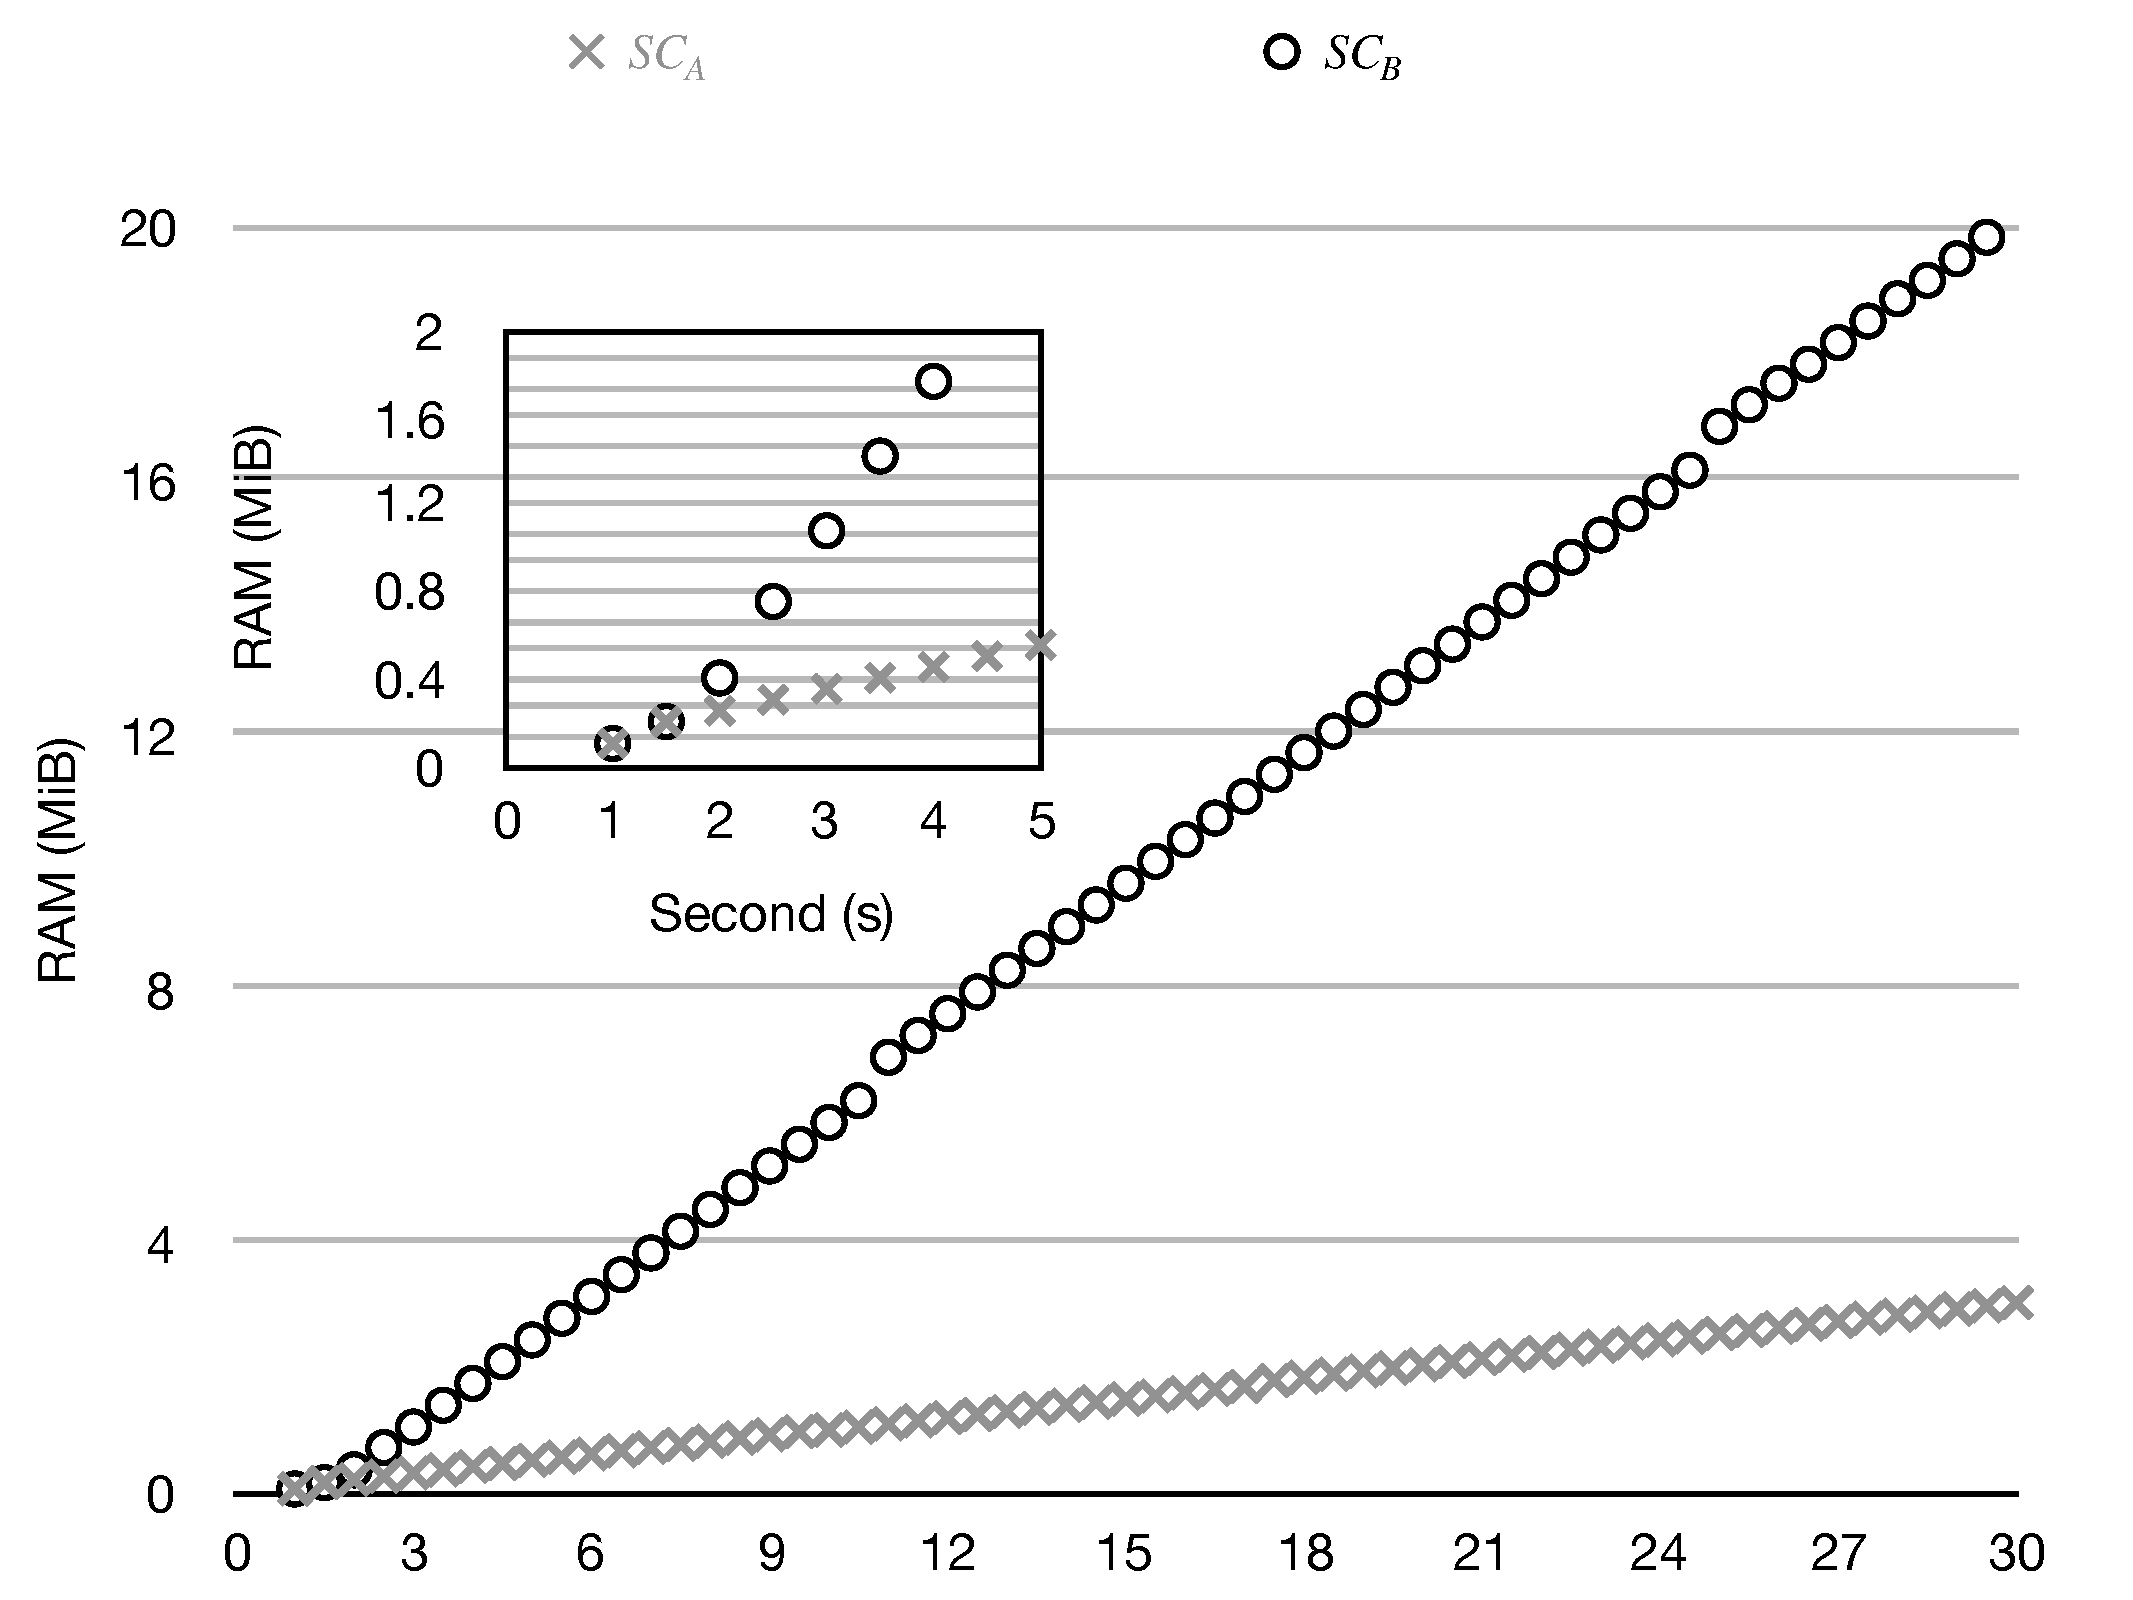
\includegraphics[width=0.8\linewidth]{figures/CREAT2.pdf}
  \caption{The amount of \ram consumed by the \SCPDOS attack.}
  %(Target SC: \texttt{danakilbock})
  \label{fig:scpdos}
\end{figure}


To conduct the attack, we implemented two additional SCs and compared their
efficacy.
%
$SC_{A}$ sends the vulnerable \SC a transaction that stores spurious data at the
\ram staked by the \SCP of the \SC. It then invokes itself via one
\texttt{send\_deferred()} call. $SC_{B}$ does the same as $SC_{A}$, however, it
invokes \texttt{send\_deferred()} twice, thus executing two instances of the \SC
at once.

\autoref{fig:scpdos} shows the experimental results. As the graph shows, the
slope of $SC_{B}$ is much steeper than that of $SC_{A}$. It only took 30 seconds
to deplete 20 MB for $SC_{B}$.
%
The actual efficacy of the \SCPDOS attack can differ depending on how much
of \ram is consumed and how the execution logic is implemented; however, this is
only a matter of time.

Once the \ram of the attacked \SCP is exhausted, the function for the \SC to use
\ram becomes no longer available.
%
Here, the \SCP can operate the \SC again by purchasing additional \ram; however,
this is only a temporary measure.
%
To sort out this problem, \SCPs should add a proper defense mechanism by
modifying the source code of the \SC and have to delete all the \ram tables
which may contain valuable user data.


\subsection{\TOCTOU attack}
\label{label_toctou}
\begin{figure}[!t] %%%1 t->h or ht
\centering
  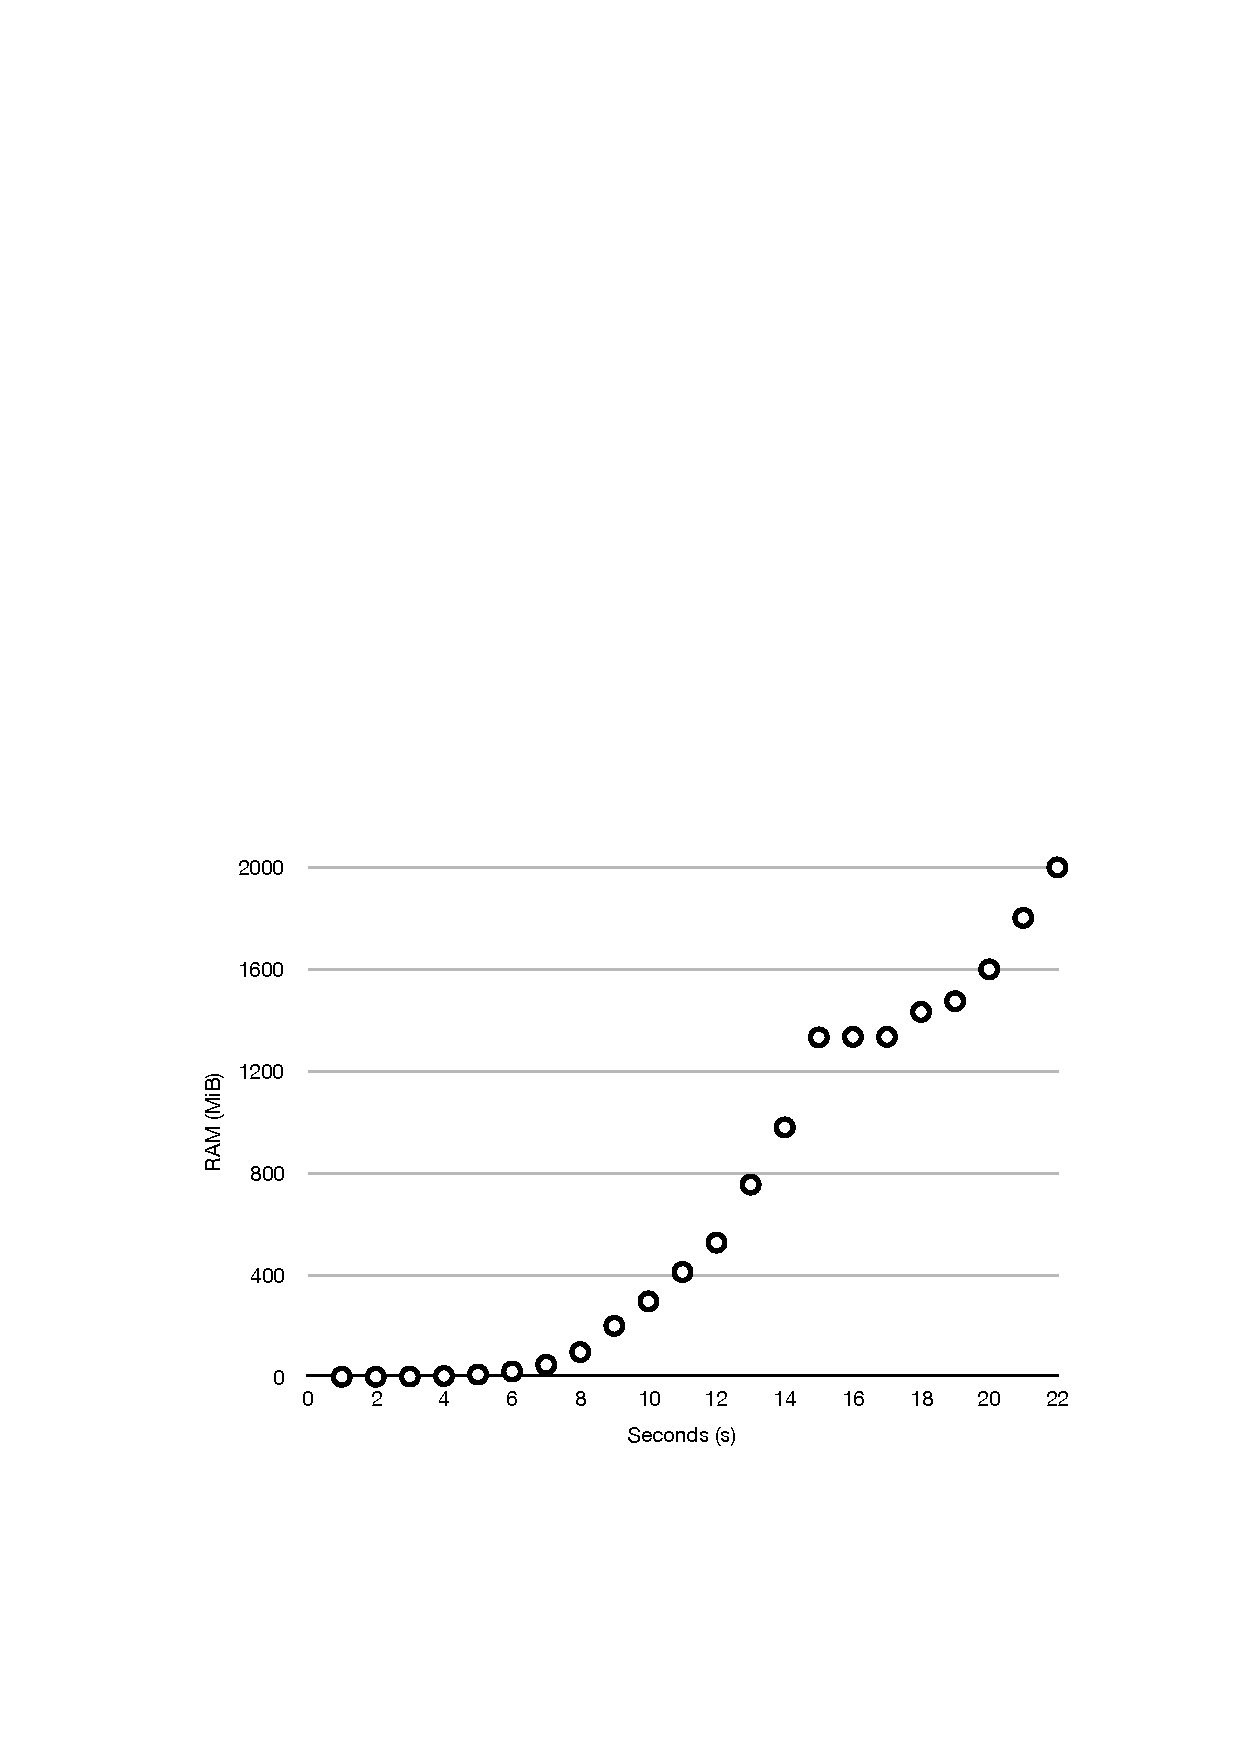
\includegraphics[width=0.8\linewidth]{figures/RAMSOMWARE_EVAL.pdf}
  \caption{The estimated \ram loss by the \TOCTOU attack.}
  \label{fig:toctou}
\end{figure}

% How attack works?`
We present the \textit{\TOCTOU} attack, a new threat that enables the adversary
to take possession of the resources of victims including \EOS tokens, \cpu, and
\ram, leveraging misplaced trust in \SCs. This attack takes advantage of the
fact that the SC of the adversary for executions can be different from the \SC
for which a victim granted the \code permission for privileged operations. This
is a classic time-of-check to time-of-use (TOCTOU) attack.

The adversary begins the attack by uploading a benign \SC. This benign \SC
requests the eosio.code permission from users for further execution.
%
As described in~\S\ref{ss:receiver}, users do not want to grant their permission
to SCPs in general.
%
In order to get the \code permission, the adversary can publish the source code
of the benign SC and obtain a safety inspection; there exist third-party
services that test the security of the submitted SCs~\cite{eospark}.
%
The adversary then promotes this benign \SC on his/her own website along with
the safety inspection results. A victim checks the published code as well as the
inspection results and decides to grant the permission to this \SC.
%
Later, the adversary switches the \SC to a malicious one, but the victim does
not recognize this change.
%
Thus, the victim is highly likely to run this changed \SC.
%
However, the \PLATFORM system does not warn or notify the victim of any code
changes made by the adversary.
%
This attack stems from the design decision of \PLATFORM that allows an \SCP to
update and revise their \SC without notifying users of such \SC changes.

One attack scenario is to lock the \ram of victims for ransom. Assuming that the
adversary is capable of obtaining the \code permission from victims, the attack
\SC can call itself repeatedly via \texttt{send\_deferred()} while storing
spurious data using the \ram of the victim until they are completely exhausted.
Unlike \cpu or \net which are restored every 24 hours, the \ram will be locked
until the adversary releases their usage. Therefore, the adversary can ask a
ransom in exchange for returning the locked \ram.

We conducted an experiment to check the feasibility of this attack in our
testing environment. We prepared a ransomware \SC and a victim account that
grants the \code permission to this \SC.
%
To fasten the completion of \ram exhaustion, we used the same methodology
described in~\S\ref{label_reentrancy-attack}, whereby the attack \SC recursively
invokes \texttt{send\_deferred()} multiple times. As~\autoref{fig:toctou} shows,
it took only around 22 seconds to deplete 2 GB of \ram, which is the \ram
capacity of the user with the most \ram when excluding the \eos
foundation~\cite{eospark}.




		\chapter{Scalability evaluation}
%Block delay attack, Ramsomware attack의 공격과는 달리 DRAIN attack 의 경우는 스마트 컨트랙트상의 취약한 패턴의 로직이 존재 하여야만 공격이 성공 하는 것을 알수 있다. 때문에 이러한 패턴의 스마트 컨트랙트가 얼마나 많이 존재하는지를 확장하여 평가 하기 위해 아래와 같은 scalability를 고려한 evaluation tool을 개발하였다.
The Resource drain attacks are supposed to have patterns of vulnerabilities unlike Block delay attack, and Ramsomware attack. thus, In this section, we introduce our scalability evaluation tool that we called E-SCV(Evaluation Smart Contract vulnerability) for evaluating how many smart contracts are undered our attacks.   


%블럭체인에 smart contract는 튜링컴플릿한 언어로 만들어진다. 때문에 일반적인 Program Language Theory를 적용 시켜 분석을 할수가 있다. 웹어셈블리어를 디컴파일 하기 위해 나온 Wasmdec\cite{wasmdec}와같은 오픈소스들이 존재한다. 그러나 이러한 오픈 소스들은 EOS smart contract용으로 디컴파일을 제대로 수행해 주지 못하였다. JEB 의 webassembly 디컴파일러\cite{JEB} 모듈을 활용하여 웹어셈블리어를 효율적으로 컨버팅 해 줄 수 있었으나 오픈 소스가 아니기 때문에 소스코드 수정을 하거나 다른  such as Symbolic execution, static taint analysis or general data flow analysis 분석 도구들을 활용하기가 어렵다.

%때문에 우리는 EOS Smart contract를 분석할수 있는 프레임워크를 직접 제작하 였고 이를 Eos Smart Contract vulnerability Auditor(E-SCV) 라고 명명하였다.
%우리는 web assembly 스마트 컨트랙트를 파싱하여 분석하기 용이한 자료 구조 형태로 저장 하였고 이를 waskCook이라 명명했다. E-SCV는 wastCook을 활용하여 web assembly 코드를 syntax가 유지되는 상태의 C 형태로 re-construct 해주는 코드를 만들어주고 우리는 이를 EOSRAY라고 불렀다. EOSRAY에 대한 제세한 설명은 EOSRAY subsection에서 다룬다. 이렇게 만들어진 자료형을 가지고 취약점까지 도달 여부를 자동으로 검출 하기 위한 분석을 진행한다.  E-SCV에서는 자료구조 형태로 만들어진 EOSRAY의 데이터를 가지고 코드를 basic block 단위로 나누고 Control Flow graph(CFG)를 형태로 변환 후, Symbolic execution\cite{Symbolic_execution}을 이용하여 실제 버그까지 도달하고, 인자 조작이 가능한지 판단한다. 이 외, 도달된 버그가 취약하게 영향을 미칠 수 있는지 Bug-Oracle 과정에서 검증한다.

Blockchain smart contracts are made by the Turing complete language. Which means that we are able to analyze a smart contract using a program language theory. There are already a few open-source projects to analysis such as  Wasmdec~\cite{wasmdec} to analysis web-assemblies. But every open source is not good at analysis to web-assembly-smart-contract. JEB company, which is one of the famous de-compiler, give to tools for web-assembly de-compile. It is nice tools, but that is closed source and paid source code. That means, we hard to use this tools for various other analyzer tools such as Symbolic execution, static taint analysis~\cite{taintAnalysis} or general data flow analysis.
For figure out these problems, we directly make a framework for web-assembly smart contracts, we called this framework as E-SCV(EOS Smart Contract Vulnerability Auditor). E-SCV is consist of two parts modules, one is EOSRAY, The other one is Analyzer. First, EOSRAY parses web assembly to data structures types. We called this parser and arrange-class to the wastCook. The wastCook re-construct web-assembly to C-level pseudo codes. We talk about detail implementation in EOSRAY sub-section. The wastCook made data structures, that are coming from the web-assembly smart contract to analyzer modules. The analyzer modules analysis to automatically find reachability to sensitive functions wastCook's data. E-SCV translate data-structures from linear codes to basic-blocks, and re-design to control flow graph(CFG). We could solve every code's expression using symbolic execution ~\cite{Symbolic_execution} to check that input values are able to reach sensitive functions. But SMT remains in future works. We do talk about analyzer's implementation in ANALYZER sub-section. After that, we will also show you verify systems for bugs what we find in the Bug oracle sub-section.

\begin{figure}[!h] %t->h or ht
  \centering
  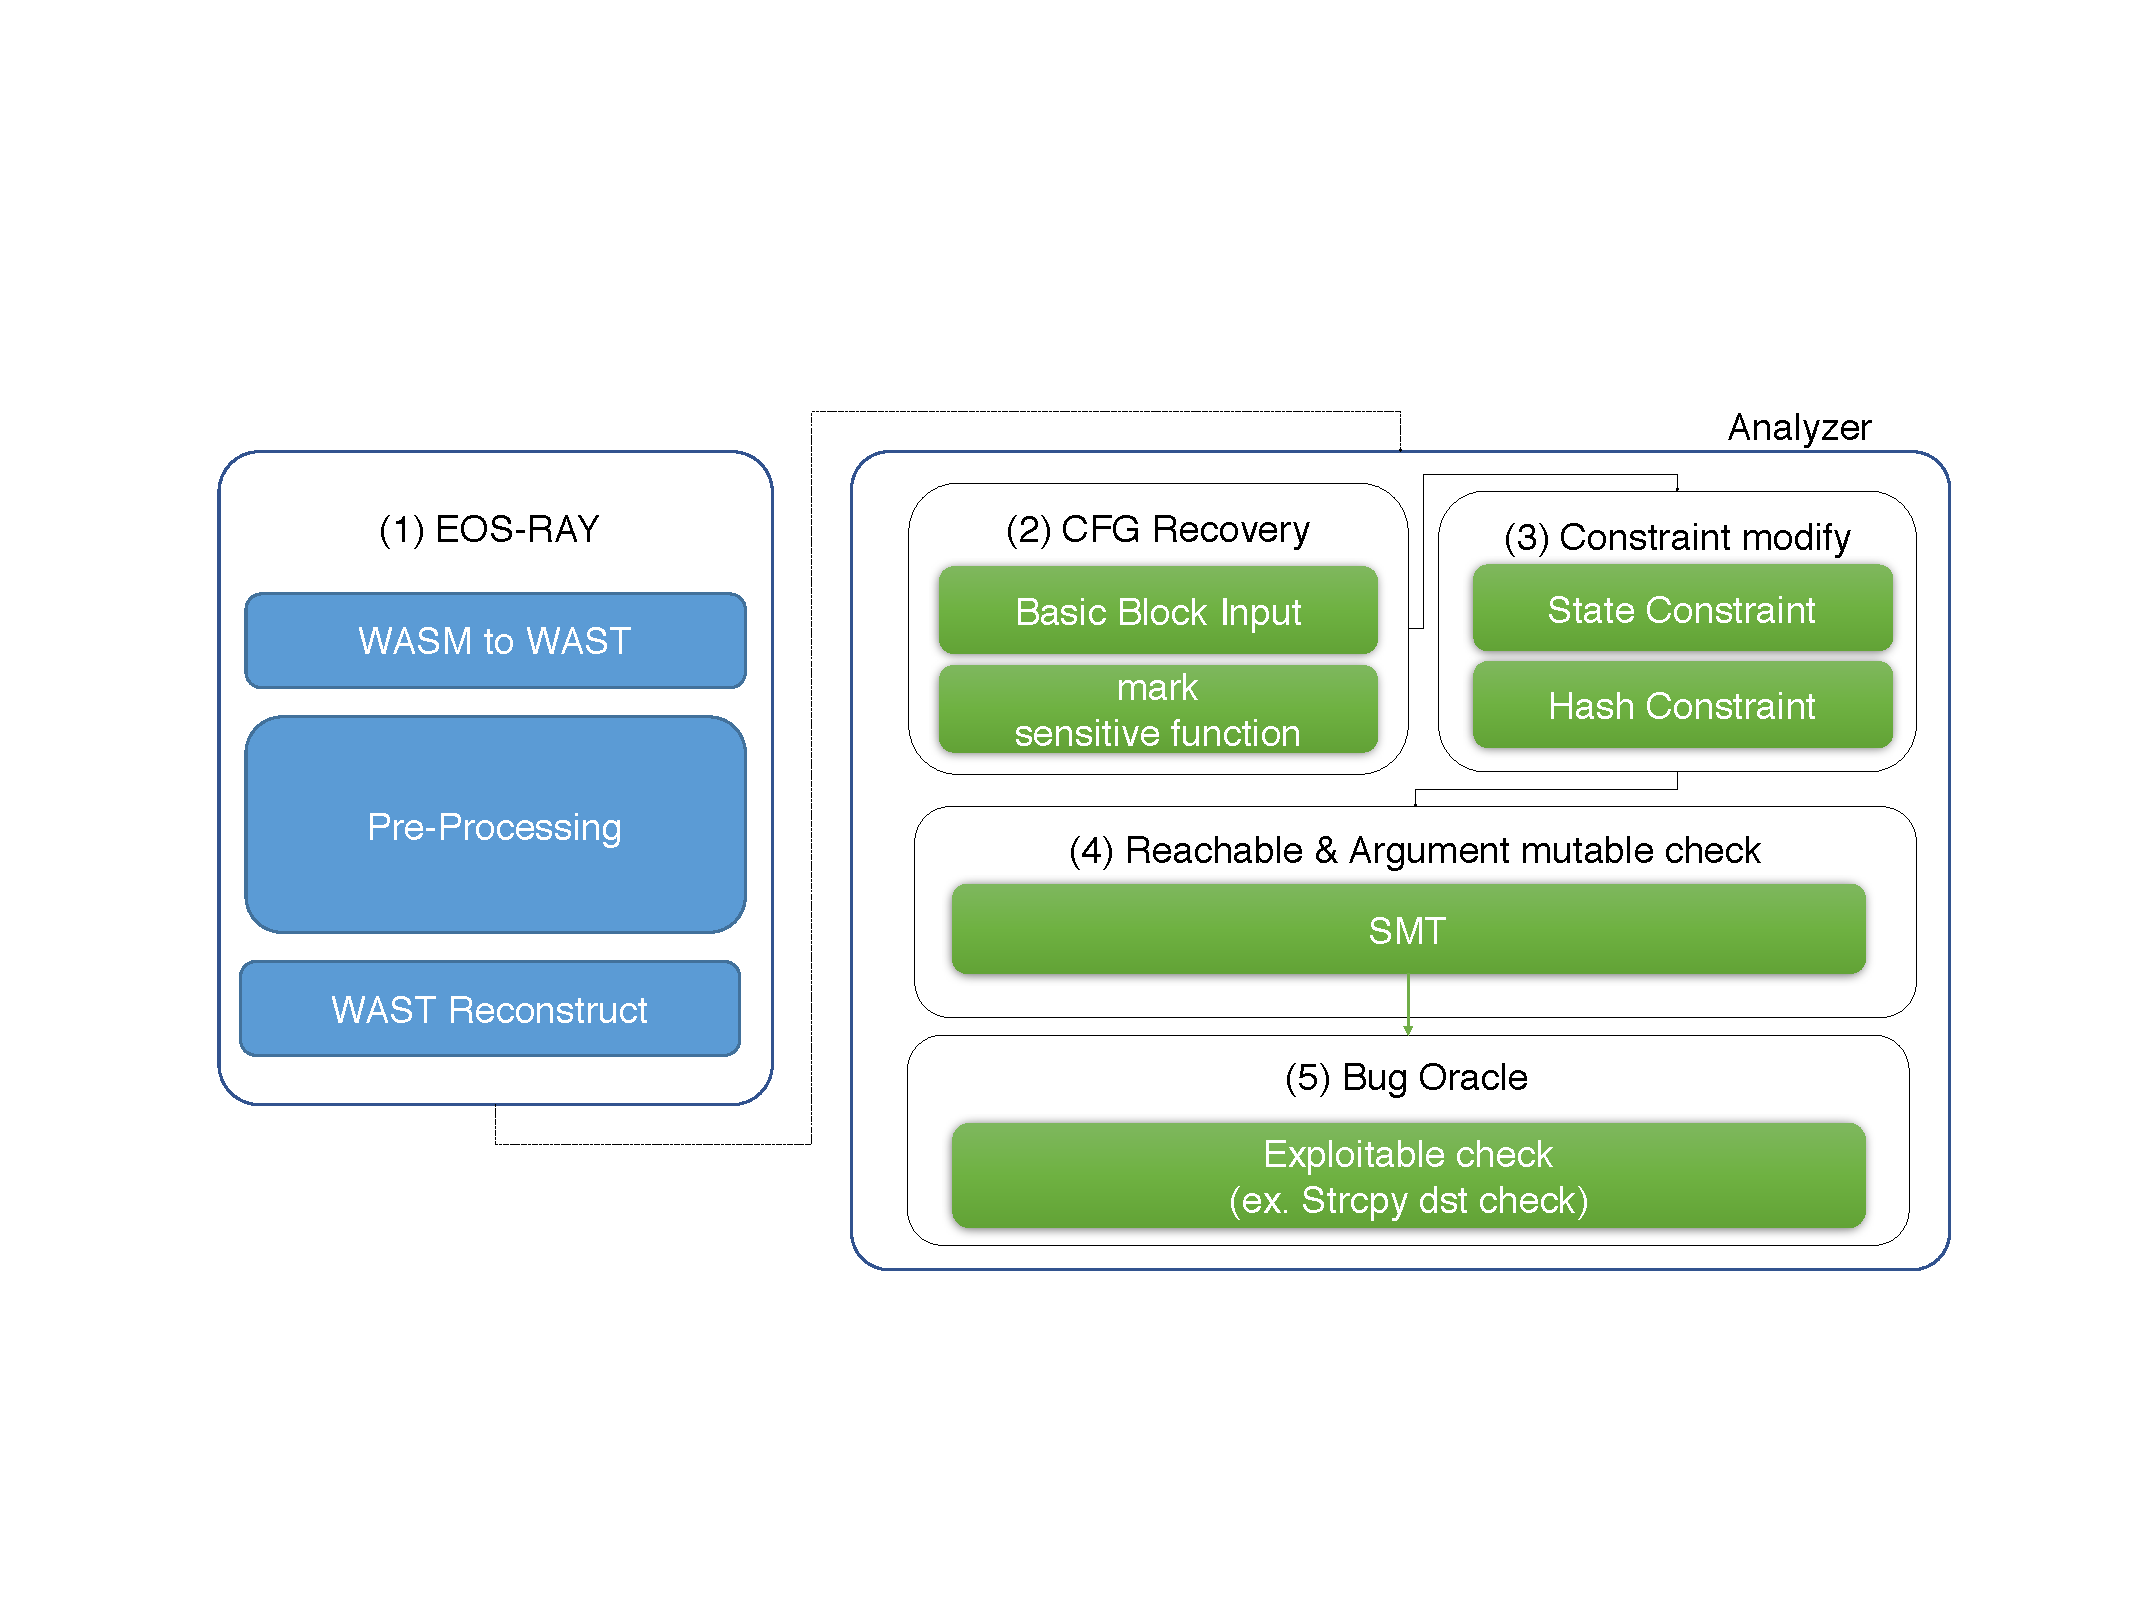
\includegraphics[width=\linewidth]{figures/scalableval.pdf}
  \caption{E-SCV Architecture}

\end{figure} 


%SEED로 사용할 스마트 컨트랙트를 모아야 할 필요가 있다.
%BP Nodeos의 패킷을 분석해 본 결과  "/v1/chain/get\_raw\_code\_and\_abi" 라는 URL 로 producer 의 계정 정보를 보내면 BP nodeos는 자신에게 해당 producer이름으로 등록되 어있는 스마트 컨트랙트와 Abi 를 반환해 준다. 
%eospark 사이트로부터 컨트랙트 1700개 를 수집 할 수 있었으며 관련한 abi도 같이 크롤링 할 수 있었다. 수집된 abi는 컨트랙트의 external method 와 method argument type을 JSON 형식이 아닌 바이너리 형태로 저장하고 있었다.
%json 파일 안에는 "structs" key 를 바탕으로 "name" 과 "fields" value 가 존재하고 "name" value 는 method를 의미하며 "fields" 는 method에 들어갈 type 을 정의하고 있다. 
%"fields"에는 int, account, asset, string 형이 존재하며 이 타입이 맛지 않은 상태로 메소드를 호출 할수 없다. 
%우리는 이러한 external method 들중 action으로 구분되어 실제 이벤트를 실행 할수 있는 함수들 선별하고, 그에 맞는 argument type을 자동으로 파싱하고 값을 대입하여 자동으로 다양한 SEED 컨트랙트의 모든 메소드를 호출 시키도록 구현 하였다. 이렇게 모든 메소드를 호출 시키는 이유는 메소드가 다른 내부 api들을 호출 하는 트리거 포인트가 된다.
\section{Crawling EOS Smart Contract}
We have collected web assembly smart contract for use as seed files.
We also do analysis BP Node's packets. and we got method for collecting smart Contracts from producer name using "get\_raw\_code\_and.abi" URL which returns smart contracts and Abi files when receiving producer ID. As a result, we can get 2960 web assembly Smart Contracts from the Eospark web site. not only smart contracts but also Abi files that exist with binary types, not JSON formats. 
there is various information for calling methods in an ABI file as dictionary styles. Action type includes callable function list, and Structs have arguments types which are consist of Names, Fields. Name field means a Method name, Field field means a type of arguments.
Fields are consist of "int", "account", "asset", "string" and so on. client have to call methods with correct fields types. So, we extract callable methods name from an action field and make correct arguments from struct fields from struct field automatically. This progress is needed for trigger method and runs API correctly.

%node 에서 가져온 ABI 파일들은 사람이 읽기에 부적합 하다. 
%우리는 이 바이너리 포멧파일에서 앞서 필요한 method 이름, argument 타입정보등을 가져오기 위해 데이터를 카빙하여 JSON 형태로 변환 해 주었다.
%바이너리 포멧의 ABI 파일의 특징은 아래와 같다.
\section{Regulating binary format ABI to JSON format ABI}
ABI file which is coming from BP Node is not readable. 
We extracted data which is needed for calling external method from binary format ABI. such as method Name, argument types. and we transform this data to JSON file format. 
We analysis the binary format and the pattern is below.
%ABI 바이너리 파일을 hex로 열어보면 특정 규칙이 존재한다.
%ABI파일의 제일 첫 1-byte는 버전 정보에 대한 길이 값을 가지고 있다.
%버정 정보를 알아 오기 위해서는 그 길이 값 만큼 다음 바이트를 읽어야 한다.
%이렇게 한바이트에 길이 값만큼 문자열을 읽어 오는 방식의 패턴화 하고 \textit{ Carving[Target]} 라고 부르도록 하자.
%버전 정보의 이름값 바로 뒤에 1바이트는 structs 에 대한 갯수 값이 들어 있다.
%우리는 앞서 구한 횟수만큼 반복하며 \textit{Carving[StructsName]} 방식을 사용 하여 모든 Structs Name 들을 가져 올수 있다. 각 Structs Name 값은 각각의 Field를 갖게된다. 
%를 위해 \textit{Carving[StructsName]}의 다음 바이트에는 각 "structs" Name 의 Field의 갯수를 저장하고 있다. 우리는 기 Field 의 갯수 값을 읽어 반복문을 돌며 \textit{Carving[StructsField]}를 통하여 필드값들을 저장한다.
%Structs Name 이 끝나고 나면 다음은 Action Name 값이 온다.
%Action Name도 structs 와 마찬 가지로\textit{Carving[ActionName]}을 진행하게 되는데 특이한 점은  Action에 대한 값은 앞에 16byte의 헤더가 붙고 17byte 째때 action Name 의 길이 값이 저장된다. 때문에 16 bytes offset 을 가진뒤 데이터를 읽어오면된다.
%다음은 Table 부분이다. 
%Table section도 Action과 마찬가지로 16byte의 헤더를 가지며, \textit{Carving[TableName]}을 통하여 값을 가져올 수 있다.
%각각의 테이블들은 여러개의 Key name들과 key type들을 가지기 때문에 TableName 바로 다음 바이트에 테이블의 type과 name을 위한 리스트의 갯수가 저장된다. 
%여기서 얻은 리스트의 갯수만큼 반복문을 돌며 \textit{Carving[KeyName]}, \textit{Carving[KeyType]}을 통해 값을 가져올 수 있다. %이후 Key Type 을 위한 name 값이 저장되어 있는데 이 또한 갯수만큼  반복문을 통하여 \textit{Carving[KeyTypeName]}을 통하여 가져 올 수 있다.
%이렇게 얻은 데이터를 가지고 개발자에게 친화적인 개발 당시 JSON형태로 복원 시킬 수 있다. 

ABI binary file has a specific file format. you can analysis using hex-editor. 
The first byte which is in the ABI file has length of the version string. We can get version string from ABI file reading length byte's size. This method which read specific size for the string is shown repeatedly. and let's called this pattern  \textit{ Carving[Target]}. Right after version information string, there is "structs"'s a number value. We can get all the "struct" names using the \ textit {Carving [StructsName]} method by Repeating the number of times previously obtained.
Each "struct" Name value has its own Field.
Because of this, After \textit{Carving[StructsName]} 1 byte has values of numbers which mean Field count. we can get all "field" names using the \textit{Carving[StructsField]} method by repeating the number of times previously obtained. 
After "struct" name comes "action name". 
An "action" name is like similar to a "struct". we can get an "action" name with \textit{Carving[ActionName]}, but there is a difference which has a 16-byte header. so after 16-bytes, there is "action" name string.
the next format is "table".
A "table" part also have 16-bytes header, and we can get "table" name string using \textit{Carving[TableName]}.
Each table has a number of key names and key types. to express this. tableName format next byte is count value for types, names. With same method before, we can get all "type" value and "name" value using the \textit{Carving[KeyName]} and \textit{Carving[KeyType]} method by repeating the number of times previously obtain number. Next byte is name for "key type" it also could get using \textit{Carving[KeyTypeName]}.



\section{EOSRAY}
%%%%%%%%%%%%%%% 모든 설명은 현재형 %%%%%%%%%%%%%%%%%%%%%%%%%%
% 왜 필요 한지에 대한 설명 (Why)
% 어떠한 방식으로 설계되었는지 설명. (How) 
% 어디에 쓰일 것인지에 대해 설명 (What)
%%%%%%%%%%%%%%%%%%%%%%%%%%%%%%%%%%%%%%%%%%%%%%%%%%%%%%%%%%%%%%%%%%%%
%WASM 파일을 분석하는 프레임워크를 만들기 위해 분석하기 어려운 WASM 바이트 코드의 형태를 분석하기 좋은 WAST 형태로 변형 시키켜야 했고, 이를 위해 EOS SDK에서 제공하는 WASM-DIS 파일을 사용하였다. 
%WASM-DIS파일은 바이트 코드 형태의 WASM파일을 WAST형태로 변형시켜 준다. WAST 파일은 좀더 개발자 친화적인 어셈블리 코드로서 우리는 이 WAST파일을 시작으로 분석툴을 개발 하였다. WAST 파일은 크게 8개지 타입으로 이뤄져 있다.;export, import, type, elem, data, global, function and call instruction.
%항목 타입 들중 function은 메인 코드가 들어 가 있는 항목이다. 이 메인코드는 stack machine 기반으로 처리 하기 좋은, 형태로 되어 있다. E-SCV는 이러한 코드들을 연산 순서 기준으로 스택 구조로 가지고 코드를 에뮬레이팅 하듯 순차적으로 처리를 하며 C언어 형태로 변환한다. 이때 각 분기를 구분하기 위한 label을 추가로 스택에 집어 넣고, label 별로 블럭을 나누어 코드로 표현한다. 이러한 변환을 위해 E-SCV 코드 내에는 웹어셈블리의 172개 instruction을 모두 C언어 형태의 문법으로 재정의 했다. C언어 문법의 형태의 연산자는 Analyzer section의 Symbolic execution에 input값으로 활용된다.  EOSRAY의 중간 산출물은 C언어 형태에 가까운 pseudo code가 되며 이러한 pseudo code를 기준으로 취약점 검증을 수행 할 수 있었다.
We need to change WASM-file to WAST-file that is a more convenient type for analysis. We used WASM-DIS binary file that is given by EOS foundation for converting. There are 8-types in web assembly; export, import, type, elem, data, global and function. Among them, main source codes are inside function type, and action-method-functions are being inside elem type. We re-defined all web-assembly instructions, which are 172 instructions, to C-level pseudo codes so that we can follow control flow from a function of elem to end of that functions. The C-level pseudo codes include various expressions. The various expressions are used to the symbolic execution's input value, and we talk about this Analyzer sections.

\section{Analyzer}
%스마트 컨트랙트의 취약점의 기준은 외부에서 입력된 데이터가 취약한 함수 까지 도달을 하는지를 보는 것이 핵심이다. 실제 취약한 함수가 존재하더라도 사용자에 의해 트리거 될수 없다면 이는 취약한 컨트랙트가 아니다. 이를 자동으로 판단하기 위해 E-SCV는 EOSRAY에서 만들어진 자료구조를 활용하여 취약점을 자동는 알고리즘을 적용하기 좋은 자료구조 형태로 변환한다. 변환된 자료구조는 Symbolic Execution을 통하여 모든 code coverage를 측정하고, 외부에서 입력 가능한 input data를 미지의 변수로 두고 민감한 민감한 함수로 sink 할 때까지 조건식들을 계산하여 외부에서 들어올 수 있는 데이터 인지 아닌지에 대해 판별하게 되며 구체적인 구현은 subsection에서 위 그림과 같은 순서대로 설명 할 것이다.
% 왜 필요 한지에 대한 설명 (Why)
% 어떠한 방식으로 설계되었는지 설명. (How) 
% 어디에 쓰일 것인지에 대해 설명 (What)

The main standard point that decides a bug is that data reachability. Which means that if the sensitive function exists in the function without input data, it is not a bug. thus, E-SCV makes Control-flow-graph(CFG) base on basic block units to the tree data-structure shape. After that, E-SCV mark function's arguments and track the arguments every single step. If the argument reach branch, E-SCV judge reachability using taint analysis. This process is terminated when arguments reach the leaf node or sensitive function. 

\section{CFG recovery}
%control-flow-graph(CFG) recovery는 일반적인 프로그램 자동 분석 시스템에서 자주 사용되는 기법이다.  이렇게 만들어진 각각의 베이직블럭의 자료구조에는 각 블럭에서의 변수값의 변위를 tracking할 수 있도록 저장하고 있고, 각 블럭별 코드에서 사용된 코드들의 연산들을 일괄적으로 관리 하고 있다. 
Control-flow-graph(CFG) recovery is used to automatic analysis for binary programs. It makes we are able to find whole code-coverages. teTher~\cite{krupp2018teether}, which is ethereum audit tool, also use this method. We adopt the CFG recovery methodology to web assembly smart contract, and it is base on the basic block tree. E-SCV build the basic-block-tree with expressions what is used each basic blocks.


\begin{table}[!t]
\caption{Estimated insecure stmart contracts}
\label{escvTable}
%\begin{center}
\begin{tabular} {ccccccccccc}
\hline\hline
& & send\_dereffered[] & db\_store\_i64[3-5] & db\_update\_i64[\^1][2] & memcpy[2] & strcpy[2] \\
\hline
& $Total API calls$	& 790 	&  	8,059	& 11,620	& 205,033 	& 63	&\\
& $Reachable APIs$	&  117 	&	11		& 7			& 393		& 1		&\\
\hline\hline
\end{tabular}
\begin{tablenotes}
\item Total: 2960 smart-contracts
\item "[num]" means that argv[num] reachability
\item "[\^n]" means that All argument except argv[\^n]
\end{tablenotes}

%\end{center}

\end{table}


\section{Reachability}
%각 Basic Block 단위로 나뉘어진 PATH를 이용해 취약한 함수가 마킹된 블록에 도달이 가능한지 확인하고, 해당 함수가 유저에 의해 조작이 될 수 있음을 확인해야 한다. 
%따라서, 함수가 포함된 블록부터 엔트리 함수까지의 경로에 저장된 Constraint를 Depth First Search(DFS) 알고리즘으로 구한 뒤,
%각 블럭을 순회하는 기준은 Depth first search(DFS) 기준이며, code의 flow가 정의된 취점에 민감한 함수에 도달 할 경우, back-tracing 을 하며 지금까지 거쳐왔던 노드들의 자료구조에 저장된 변수들과 연산자들을 계산하며 빠져나오게 된다.
%satisfiability-modulo-theories(SMT) Solver의 조건에 스택 형태로 삽입 하여 풀이 함으로써 우리가 넣은 어떤 인자에 의해 조작되는지 알 수 있다. 즉, 엔트리 함수, 취약 함수, 인자 번호, 영향을 미치는 입력 값 쌍에 대한 정의를 함으로써 버그 오라클 과정에서 사용될 데이터를 만들어낼 수 있다.
% 엔트리 함수, 취약 함수, 인자번호, 영향을 미치는 입력 값 세트 수식 형태 예시 만들 수 있을듯?
After re-constructing, E-SCV has to mark the function's arguments and track the arguments every single step and make sure reachability to sensitive functions and argument manipulatable via users. Therefore, E-SCV calculates every instructions and data along to constraint-path as Depth First Search(DFS) method. If the code flow can be reached to sensitive functions, E-SCV could solves conditional equations using satisfiability-modulo-theories(SMT) Solver, while back-tracing every basic block with saved variables and expressions but this part is not implemented yet. For now, Only thing have is input reachability to sensitive functions using taint analysis.


% send_dereffer(), db_update_i64, db_store_i64, memcpy etc... 
\section{Sensitive Functions}
The send\_dereffer() API use EOS-CPU which has to staking EOS coin. So, To reduce unnecessary waste of resources, If the developer wants to use send\_dereffer() APIs, s/he is supposed to set authorization for using its. db\_update\_i64() and db\_store\_i64() are also have to set strict ram-payer for preventing overcharge EOS-RAM which has to purchase by not only attacker but also benign users. This is just the developers mistake. so we evaluated how many smart-contracts that have mistake is being in real EOS-ecosystem using E-SCV.

\section{Limitation and Evaluation}
%이러한 방법론에는 두가지 제한 사하잉 있다. 하나는 상태조건에 따른 함수들의 제한이 있을때이며, 두번째는 두개의 context흐름 서로 유기적으로 연결되어 있을때 이다. 

%예를들면 smart contract에 저장된 데이터를 불러와서 그 값에 의해 취약한 함수가 트리거 되는 케이스이다. 이 경우에는 외부에서 전달되는 값이 직접적으로 취약한 함수로 전달되지 않기 때문에 위 방법으로는 탐지가 되지 않는다.

%두번째는 sensitivie function에 인자가 도달하지만 특정 조건을 만족(컨트랙트에의해 허가된 사용자)하거나 값을 검사하는 로직이 
%pre-condition에 존재하는 경우는 문제가 없는 데이터만 전달 되기 때문에 취약하지 않다. 이러한 검사 로직에 어떠한 것들이 존재하는지 확인하고 condition을 만족하는지를 판단해야만 하지만 아직 그에 따른 기능을 구현하지는 않았고 future work으로 남긴다. 

These methodologies have two limitations. One is when constrained access with the condition of status. and the second case is that when each context is connected directly. 
The "constrained access" means that If the auditing-APIs that are check parameters exist before sensitive data, there is no bug from these functions, even If the external parameter reaches the sensitive-functions.To figure out this problem. we have to make a checker for checking a pre-condition but this solution remains in future works.
The "Each context is connected directly" problem is that If a function loads the data from the smart contracts database and inserts the data into the sensitive-functions then E-SCV won't get detect the bug. because the values don't directly come from the external parameters. 


%우리는 먼저 단순히 외부에서 호출되는 함수에 인자가 실제 sensitive 한 function들의 argument로 전달 되는지만을 파악하였고 결과는 표 \autoref{escvTable}와 같다. 우리는 총 2960개의 스마트 컨트랙트에서 sensitive function을 얼마나 많이 호출하는지를 먼저 단순히 찾아 보았고, 그 갯수는 TotalAPIcalls 이다. 
%하지만 sensitive function들의 모든 argument가 취약한 것은 아니다. 각 함수들은 지정된 argument에 해커의 파라미터가 전달 되는 지에 따라 취약한 함수가 된다. db_update_i64 의 경우에는 1번째 인자 ram_payer가 self로 되어있고 2번째 인자(data)를 외부에서 직접 입력이 가능한 부분을 찾아야한다. self 는 하드 코딩되어 있기 때문에, 직접 그 값을 확인 하지는 못하고, 그 self 값을 tracking 하는 것이 아닌 외부에서 전달 되지 않는 것으로 대체한다. 

We first notice that the argument is simply passed as an argument to the function that is actually sensitive to the externally called function. We first simply look at how many sensitive functions are called in a total of 2960 smart contracts, and the number is TotalAPIcalls in  \autoref{escvTable}.

However, All arguments that is pass into sensitive-functions are not vulnerable. Each function becomes vulnerable depending on whether the hacker's parameter is passed to the specified argument. In the case of db\_update\_i64, the first argument ram-payer must have "self" and the second argument which is data must be coming from the outside. However, it is hard to directly check the value is "self". thus, We check that the ram-payer is not coming from the outside instead of the value is set by "self".

%db_store_i64 역시 같은 방식으로 3번째 인자(payer)가 외부에서 들어오지 않고, 5번째 인자 (buffer)가 외부에서 들어오는 함수들에 대해서 검출한다. 
%memcpy의 경우 0번째 인자(dest)와 상관없이 1번쨰 인자(buffer)와 2번째인자 (size)가 외부에서 들어오는 함수들만을 검출하며strcpy 역시 마찬가지이다. 

%EOS-CPU, EOS-NET drain attack에 문제가 되는 send\_dereffer()의 경우에는 일반적으로 smart contract로부터 user-권한의 요청이 없는 한 contract 가 EOS-CPU, EOS-NET을 호출 하므로 send\_dereffer() 함수 이전에 require_auth 가 없는 것을 기준으로 검출하였다. 

In the same way, db\_store\_i64 detects functions from which the third argument (payer) does not come from the outside and the fifth argument (buffer) comes from the outside.
In the case of "memcpy" is that It detects that 1-argument which is buffer and 2-argument which is size is coming from the outside.
In case of send\_dereffer() which is a problem in EOS-CPU and EOS-NET drain attack,is detected based on the absence of require\_auth before the function. Because, send\_dereffer() API used to use contract's EOS-CPU, EOS-NET normally.
%우리는 위와 같은 기준으로 도달 여부를 판단하여 \autoref{escvTable}의 reachableAPI 표에 표기한다.
We determined the reachability with these criteria and the result is reachableAPI in table \autoref{escvTable}.


% send_deferred(sender_id, payer.value, serialize.data(), serialize.size(), replace_existing);
% db_update_i64(int32_t iterator, account_name payer, const void* data, uint32_t len)
% apply_context::db_store_i64( uint64_t code, uint64_t scope, uint64_t table, const account_name& payer, uint64_t id, const char* buffer, size_t buffer_size ) 



		\chapter{Mitigation}
\label{s:mit}

In this section, we propose mitigation methods for the presented attacks. We
first enumerate precautionary suggestions that require no changes to the current
\eos system. We then discuss several design changes to the \eos system to remove
the root causes of the attacks presented herein.


\section{Preventative measures against attacks}
\label{ss:simple}

The \TESER, \SCPDOS, and \TOCTOU attacks can be easily prevented if \SCPs and
users carefully inspect their \SC source code as well as the \SCPs.
%
For the \TESER attack, an \SCP should verify if the code exists in their \SC that checks the SC's callers in a manner that they cannot abuse.
%
For example, one can add a permission check at the beginning of the \SC, so that
only authorized users can use the \SC.
%
On the other hand, to prevent the \SCPDOS attack, \SCPs should carefully audit their 
\SCs to determine whether there exists code that mistakenly uses their \ram.
%
In the case of the \TOCTOU attack, a \user should give his/her permission code 
only to the fully trusted \SCPs.

These simple preventions seem to be textbook examples, and none of them requires
any change to the underlying \PLATFORM architecture. To render the system more
secure, however, we do believe that the system must do its best effort to address
threats from every entity in the system.
%
For instance, in case of the \TESER attack, the \eos system can improve its security by
adding extra security components to it.
%
This approach is not uncommon as one of the largest systems, a Linux kernel,
adopted a similar concept to alleviate the threats derived from mistakenly
omitted permission checks~\cite{mcclure2009hacking}.
%
In the following subsections, we discuss potential changes to the \eos system to
fundamentally eliminate the root causes of the attacks presented above.

\section{Shifting the payment responsibility}
\label{ss:shifting}

As described in~\S\ref{label_teser}, in the \TESER attack, a malicious user intentionally
triggers a target SC to deplete the \cpu of its SCP. Of course, an SCP can
prevent this by carefully inspecting the code of their SC. However, this attack
stems from the current design that encourages \SCPs to pay for the execution of
their \SCs originating from user transactions.

In the current \eos system, to impose the transaction cost on a specific user,
an \SCP has to specify the user as authorized in the \SC, and this process
requires the \code permission from the user. In general, users are not normally
willing to grant this permission code since anyone with the code is able to
control the user account.
%
To avoid this, an SCP is supposed to create an SC with his/her own permission
code that imposes the transaction cost of executing the SC onto the SCP
himself/herself so that any user can be pleasant for the execution of the SC
without providing the permission or paying the cost.
%
Therefore, our design change suggestion removes the constraints of SCPs, thus
enabling them to avoid using their own resources, which also eliminates the
target of the attacker.

One way to address the \TESER attack could be to redesign the \eos system so that a user
who initiates a transaction should pay the transaction cost without having to
provide the \code permission.
%
It is quite intuitive to impose a transaction cost on the user who actually
wants to run the SC.
%
This fundamentally eliminates the liability of checking the permission of the
SC, as well as the benefit of the attack---thus, the adversary would no longer be
motivated to commit it.

On the other hand, this mitigation increases the possibility of opposite
cases in which a malicious SC could deplete the resources of a user because it 
does not need the permission code of the user.
%
Even when the user chooses to run a malicious SC, the system should be
responsible for alleviating the severity of the threat.
%
However, as the current \eos system supports limiting the maximum resource use
for running an SC, this can be mitigated as well~\cite{resourcemaxusage}.

\section{Fine-grained permission control}
\label{ss:fine}

The root cause of the \TOCTOU attack is a user giving his/her permission code
(\code) to an SCP in the belief that the SCP will not abuse this permission.
This, in fact, can be considered the fault of the user as s/he gives permission
with full awareness of the significance of their action. Nevertheless, the \eos
design can be changed to protect users from these kinds of threats.

Currently, the \eos permission system pursues an all-or-nothing
approach. That is, a user can make only one kind of action regarding his/her
permission---either give or revoke it.
%
This fundamentally facilitates threats on assets in \eos, including the \TOCTOU
attack.
%
The \eos developers are also aware of this issue and have proposed pinning
the permission into a specific version of the target SC. However, this still remains
an unresolved issue~\cite{EOSEOSIOCODE}.
%
Nevertheless, we have proven the feasibility of this threat, as shown
in~\S\ref{label_toctou}, and here we suggest possible mitigation that can eradicate
such threats.

We propose a fine-grained permission control, including the permission pinning 
described above. It enables a user to set a specific period or a specific
version that the permission depends on. As a result, in case of the 
\TOCTOU attack, even though a malicious SCP replaces a benign SC with a 
fraudulent one, the given permission would automatically lose its validity. 
Moreover, the expiration date of the permission can reduce the feasibility of 
the threats occurring because a user might forget to revoke permission.
%
Therefore, the fine-grained permission control can help to mitigate several
threats to the \eos assets.

		\chapter{Related work}

%To the best of our knowledge, no research has analyzed the risk of \PLATFORM
%architecture. Several studies focused on inspecting the \ETHER's \SC
%vulnerabilities and blockchains, and There are some \PLATFORM's vulnerabilities
%on online. The system architecture of \PLATFORM's features across different
%environments with other blockchain platforms

%\subsection{블록체인에서의 취약점 연구 사례}
%\ETAL
% [합의 알고리즘] I. Eyal \ETAL \cite{eyal2018majority}: Selfishi mining [합의
% 알고리즘] I. Eyal, "The miner's dilemma", IEEE S&P'15: BWH 공격 얘기.. [합의
% 알고리즘] Y. Kwon, D. Kim, Y. Son, E. Vasserman, Y. Kim, "Be Selfish and Avoid
% Dilemmas:Fork After Withholding (FAW) Attacks on Bitcoin", ACM CCS'17: PAW
% 공격 얘기..

% [블록체인을 운영하는 노드를 공격함.] E. Heilman, A. Kendler, A. Zohar, S.
% Goldberg, "Eclipse Attacks on Bitcoin's Peer-to-Peer Network", USENIX Sec'15

\section{Security analysis of blockchain systems}

Many previous studies have investigated the security of blockchain
systems~\cite{\bcPapers}. Most of them focused on analyzing the two blockchain
systems; \btc and \eth.
%Here, we introduce a few of them.
%
There is a large body of work on \btc attacks. Researchers have analyzed 
double spending~\cite{karame2012double}, network-related attacks~
\cite{heilman2015eclipse, apostolaki2017hijacking}, illicit transactions~
\cite{son2019ndss}, transaction malleability~\cite{decker2014bitcoin,
andrychowicz2015malleability}, and selfish mining~\cite{\miningpoolPapers}.
%
Eyal~\etal~\cite{eyal2018majority} introduced a selfish mining problem in
which rational \btc miners collude to control the entire \btc system, including 
taking over the mining profit.
%
Heilman~\etal~\cite{heilman2015eclipse} demonstrated the eclipse attack on the 
\btc network where  an adversary can fabricate \btc mining power by spoofing the 
routing tables of other miners. They utilized this to conduct double spending attacks as well.
%
Kwon~\etal~\cite{kwon2017selfish} proposed the fork-after-withholding attack,
in which selfish miners secretly keep new blocks as long as possible to maximize
their profit.

Previous research has also investigated the security of \eth smart contracts~
\cite{\smartcontractAll}.
%
Luu~\etal~\cite{luu2016making} introduced an automatic bug finding tool for \eth
SCs. They aimed to discover bugs that allow colluding miners to intentionally 
reorder the execution of SCs or to change the timestamp of SCs.
%
They also presented the notorious re-entrancy bug, which allows an adversary to
continuously execute a target SC for various purposes.
%
Krupp~\etal~\cite{krupp2018teether} developed a tool that
automatically generates exploits for identified SC vulnerabilities, and
Kalra~\etal~\cite{kalra2018zeus} presented another tool that automatically
remediates a target \SC by inserting security checks.
%
%There have been other open-source tools~\cite{\smartcontractTools} as well.

Recently, researchers have started analyzing the security of other blockchain
systems, such as Ripple~\cite{rippleattack},
Monero~\cite{hinteregger2018empirical, moser2018empirical}, and
Stellar~\cite{kim2019is}. In addition, there have been studies on evaluating
various consensus algorithms~\cite{zhang2019lay}, and analyzing the decentrality
in permissionless blockchains~\cite{kwon2019impossibility}.

In line with this research, we analyzed the \eos system an identified new security concerns that are rooted in the unique characteristics of \eos and also described their attack scenarios.
%
We are planning to develop an analysis platform for \eos SCs, following the
previous papers~\cite{luu2016making, krupp2018teether}.


\section{Security analysis of \eos}

Even though there exist many studies on \btc and \eth, there have been only a few studies conducted on \eos. 
%
%In fact, we tried to find other academic papers on the security of \eos, but we were unable to find even one. Here, we introduce several bugs~\cite{\eosBugs} found in the industry.
We only found several bugs~\cite{\eosBugs} reported from the industry.
%
These bugs can be categorized as software bugs in the core \eos system
~\cite{\eosSoftwareBugs}, logical bugs in \eos SCs~\cite{\eosSCBugs}, and a
design bug~\cite{\eosDesignBugs}.

Chen~\etal~\cite{EOSARBITCODE} found an arbitrary code execution bug in \eos.
This bug is essentially caused by an integer overflow bug when executing an SC
that leads to out-of-bound buffer access.
%As a result, an adversary could take over the control of the nodes.
%
There are bugs from mis-implementation of SCs as well~\cite{\eosSCBugs}. One
example is that an adversary can exploit an SC that does not properly check the
caller of the SC, allowing multiple \eos SCs to be executed
subordinately~\cite{requireRecipient}.
%
The third category is a bug that stems from the \eos core design, allowing a
large number of transactions to delay the block creation time~\cite{eosNodeDoS}.
This appears to be similar to our \NODEDOS attack; however, they essentially
differ in that the \NODEDOS attack pauses BPs by exploiting their transaction
scheduling algorithm. Hence, it can effectively break the system down.

In this paper, we documented four new threats and attacks. Even though some of
them seem trivial,  their underlying causes are related to the \eos system
design. We also addressed specific design concerns with the current \eos system
and noted how fixing them would address potential threats to \eos.

		\chapter*{Conclusion} %Don't want chapter number for conclusion

Building a secure system demands an understanding of potential threats and their 
underlying root causes.
%
We conducted the first study that analyzes the security of the \eos system,
which has recently become one of the most popular blockchain systems. We 
presented three novel attack methods along with one concrete attack scenario, 
abusing the controversial \eos design policy. All the attacks exploit new
system components, including \cpu, \ram, and BP scheduling, which are unique to 
\eos. We also conducted the experiments for each attack, thereby demonstrating
their severities. 
%
Finally, we proposed the possible mitigations of the presented threats.

In this paper, we manually checked several smart contracts whether they are
vulnerable to the presented attacks. However, we believe there still exist
other vulnerable SCs that have yet to be discovered. We leave finding vulnerable \eos
SCs on a larger scale as a promising future work.





%%
%% 참고문헌 시작
%% bibliography
%% 위는 보기이므로 학과 또는 논문의 특성에 맞게 조정 가능함. 다만, 참고문헌마다 충분한 정보가 들어 있어야 한다.

%Bibliography
%%\bibliographystyle{splncs03}
%%\bibliography{references/refGeneral,references/reference2} %Separate multiple *.bib files with commas

{\footnotesize
	\bibliographystyle{splncs03}
	\bibliography{references/refGeneral,references/reference2} %Separate multiple *.bib files with commas
}

%%
%% 사사 시작
%% Acknowledgement
%% 사사 작성은 선택사항임
% @command acknowledgement 감사의글
% @options [1 | 2 | 3 |4 ]
% - 1 : 본문과 감사의 글이 둘 다 한글일 때  | 2 : 본문은 한글인데 감사의 글이 영어일 때 | 3 :  본문과 감사의 글이 둘 다 영어일 때  | 4 : 본문은 영어인데 감사의 글이 % 한글일 때 

\iffinal
	\acknowledgment[4]
	가장 먼저 학술연수 파견이라는 좋은 기회로 저를 KAIST로 보내주신 삼성 리서치의 황용호 랩장님께 감사를 드리고 싶습니다. 부하 직원을 발전 시키는 상사가 좋은 상사라는 말씀을 해주시며 이상섭이라는 한 사원에게 2년이라는 긴 시간을 투자해 주신 것은 단순히 존경스러운 상사를 넘어 인생의 멘토로 평생 가슴에 품고 살것 같습니다. 
	더불어 저를 선택해 주시고, 학교를 들어오기 전 부터 랩실을 마무리하는 순간까지 많은 조언을 주셨던 김용대 교수님께 특별히 감사의 말씀을 드리고 싶습니다. 
	
	둘째로 늘 창의적인 아이디어가 번뜩이는 해킹-크리에이터 (김)대준이, "논문 Writing이란 이런것이다"를 보여준 동관이, writing더불어 석사 생활의 tiping point를 만들어주신 손수엘 교수님께 무엇보다 감사의 말씀을 전합니다. 이 분들이 없었다면 너무나 많은 것을 놓치고 졸업을 했을 것 같습니다. 

	셋째로 Sysec SA팀에게 감사의 인사를 드립니다. 분야무관, 모든 과제를 케어하는 팀의 정신적지주인 동관이 부터, 늘 뛰어난 판단력과 이성적인 조언을 많이 해준 동환이, fact advisor 민근이, 모든 기술들에 대한 답을 가지고 있던 갓 해커 은수, 2년을 함께 지내며 허당인 내가 놓치는 부분을 잘 항상 챙겨 주었던 현기, 곧 회사 메신져에서 볼 요한이, 보안 모든 분야를 팔로우하는 general hacker 창훈이, 주 분야가 아닌 새로운 분야도 모든 빨리 배우고 익숙해지는 브레인 묘준이. 이들 모두 덕에 재미있고 의미 있는 2년을 보내고 졸업하게 되었습니다. 
	그 외에도 타팀이자, 나이 많은 형인데도 외면해 주지 않고 케어 해준 상욱이, 지호, 도현이, 철준이, 민철이, 호준이, 수빈이, 민정이, (권)유진이 그리고 적진 않았지만 그 외 Syssec 친구들 너무너무 고맙습니다.
	그리고 SCTF부터 DEFCON까지 좋은 추억을 만들어준 엄청난 실력+인성까지 반듯한 갓 해커들이 집합: Kaishack 멤버들 에게도 너무나 고마움을 표하고 싶습니다.
	더불어 1학년 1학기 때 같은 조별 과제로 뭉쳤다가 베스트 프랜드가 된 엘리트들, (오)동현이, 박선녀, 김홍식이! 2년 동안 마음의 안식처 같은 카톡방을 꼽으라면 단연 이친구들의 카톡방이였고 덕분에 재미있는 석사 생활을 보낼 수 있었습니다.

	마지막으로 정신적 고민의 순간에 늘 정신적 지주가 되어주신 어머니, 아버지, 그리고 힘들 때는 응원해주고 어려울때는 안식처가 되어주며 늘 옆에서 지켜준 여자친구 은이에게 무한한 감사의 말씀을 전하고 싶습니다.

	
	석사생활 동안 제가 가진 것보다 많은 것을 해낼 수 있었던 것은 이렇게 주변의 좋은 친구들 덕이라고 생각하고 있습니다.
	카이스트에서 만난 모든 분들에게 너무나 감사드립니다.
\fi

%%
%% 약력 시작
%% Curriculum Vitae
%% 약력 작성은 선택사항임. 약력 내용도 알맞게 바꿀 수 있음
% @command curriculumvitae 이력서
% @options [1 | 2 | 3 |4 ]
% - 1 : 본문과 약력이 둘 다 한글일 때  | 2 : 본문은 한글인데 약력이 영어일 때 | 3 :  본문과 약력이 둘 다 영어일 때  | 4 : 본문은 영어인데 약력이 한글일 때 

\iffinal
	\curriculumvitae[4]
		% @environment personaldata 개인정보
		% @command     name         이름
		%              dateofbirth  생년월일
		%              birthplace   출생지
		%              domicile     본적지
		%              address      주소지
		%              email        E-mail 주소
		% - 위 6개의 기본 필드 중에 이력서에 적고 싶은 정보를 입력
		% input data only you want
		\begin{personaldata}
				\name       {이 상 섭}
				\dateofbirth{1987}{07}{20}
				\email    {k1rh4.lee@gmail.com}
		 \end{personaldata}

		% @environment education 학력
		% @options [default: (none)] - 수학기간을 입력
		\begin{education}
				\item[2017. 9.\ --\ 2019. 2.] 한국과학기술원 (석사)
				\item[2007. 2.\ --\ 2013. 8.] 홍익대학교 (학사)
				
		\end{education}

		% @environment career 경력
		% @options [default: (none)] - 해당기간을 입력
		\begin{career}
				\item[2016. 3.\ --\ ~current] BoB(Best of Best) Mentor
				\item[2014. 3.\ --\ ~current] 삼성 리서치 (Security LAB)
				\item[2013. 3.\ --\ 2014. 2.] 삼성전자 (소프트웨어 멤버십 운영자) 
				\item[2011. 8.\ --\ 2012. 2.] piosoft(linkhub) - startup
				\item[2009. 3.\ --\ 2011. 4.] 공군 작전사령부 정보보호병
		\end{career}

		% @environment activity 학회활동
		% @options [default: (none)] - 활동내용을 입력
    \begin{activity}
    			%\item[2019. 08] DEFCON CTF 27 Finalist ( KaishHack )
    			%\item[2016. 2017.] 삼성전자 - SCTF 운영 및 문제 출제
    			%\item[2016. 2017.] 벨루미나 CTF (invited)
    			%\item[2013. ] KISA HDCON Finalist
    			%\item[2013. ] WhiteHat contest Finalist
    			%\item[2012. 3.] 홍익대학교 - 해킹방어대회 학과장상 수상 
    			%\item[2012. 3.] 삼성전자 - 삼성 소프트웨어 멤버십 기술면접 만점상 수상
    			%\item[2010. 3.] 공군배 - 해킹방어대회 최우수(참모총장상) 수상
    	\item 2019.08. \textit{USENIX WOOT'19 Conference Speaker}		
        \item 2019.08. \textit{DEFCON CTF 27 Finalist(KaishHack)}
        \item 2016, 2017 \textit{SCTF 운영 및 문제 출제(Samsung Resurch \& KaisHack)}
        \item 2016, 2017 \textit{벨루미나 CTF(invited)}
        \item 2014.9. \textit{CodeEngine PSD hacking Speaker}
        \item 2013.6. \textit{KISA HDCON Finalist}
        \item 2013.6. \textit{WhiteHat contest Finalist}
        \item 2012-2013. \textit{삼성소프트웨어 멤버십(대전)}
        \item 2012.3. \textit{홍익대학교 해킹방어대회 학과장상 수상 }
        \item 2012.3. \textit{삼성 소프트웨어 멤버십 기술면접 만점상 수상}
        \item 2010.3. \textit{공군배 해킹방어대회 최우수(참모총장상) 수상}
    \end{activity}
%% 학회활동을 쓰고싶으시면, 이 문서와 클래스 문서의 학회활동 부분을 사용하십시오.

		% @environment publication 연구업적
		% @options [default: (none)] - 출판내용을 입력
		\begin{publication}
				\item Sangsup Lee, Daejun Kim, Dongkwan Kim, Sooel Son, and Yongdae Kim, KAIST \textit{Who Spent My EOS? On the (In)Security of Resource Management of EOS.IO}, Master Thesis, Conference on USENIX WOOT'19 2019.
		\end{publication}

\fi

  \label{paperlastpagelabel}     % <-- 추가 부분: 마지막 페이지 위치 지정	
%% 본문 끝
\end{document}
